\documentclass[12pt,a4paper]{article}
\usepackage{amsmath,amssymb,mathtools}
\usepackage{geometry}
\geometry{margin=1in}
\usepackage{microtype}
\usepackage{caption}      % optional but recommended
\usepackage{subcaption} 
\usepackage{tikz}
\usetikzlibrary{arrows.meta}
\usetikzlibrary{calc}
\usetikzlibrary{angles,quotes}
\usepackage{enumitem}
\usepackage{float}
\usepackage{hyperref}
\usepackage{tikz-cd}
\usepackage{float}

\usepackage{pgfplots}
\pgfplotsset{compat=1.18}

\usetikzlibrary{positioning}

\usetikzlibrary{decorations.markings}

\usetikzlibrary{calc,arrows.meta,patterns,decorations.pathreplacing}
\usepackage{tikz-3dplot}
\usepackage{xcolor}

\DeclareMathOperator{\ord}{ord}

\DeclareMathOperator{\Log}{Log}


\usepackage{fancyhdr}
\pagestyle{fancy}

\newcommand{\II}{\mathrm{I\!I}}

\newcommand{\C}{\mathbb{C}}

% (optional) if you also want the first fundamental form:
\newcommand{\I}{\mathrm{I}}

\newcommand{\hyp}{\mathbb{H}}

\DeclareMathOperator{\Tr}{Tr}
\newcommand{\T}{\mathsf{T}} % transpose symbol


\newcommand{\R}{\mathbb{R}}
\DeclareMathOperator{\PSL}{PSL}

\DeclareMathOperator{\Area}{Area}
\DeclareMathOperator{\Isom}{Isom}
\newcommand{\HH}{\mathbb{H}}

\newcommand{\DD}{\mathbb{D}}

\newcommand{\n}{6}

% --- codim operator (put in the preamble) ---
\DeclareMathOperator{\codim}{codim}


\newcommand{\Solution}{\par\medskip\noindent\textbf{Solution.}\ }
\newcommand{\Theory}{\par\medskip\noindent\textbf{Theory.}\ }
\newcommand{\Proof}{\par\medskip\noindent\textbf{Proof.}\ }


\fancyhf{}

\fancyfoot[C]{\thepage}

	\fancyhead[L]{\textit{Differential Geometry 4}}
\fancyhead[R]{\textit{Exercises}}

\DeclareMathOperator{\arsinh}{arsinh}

% --- HEADER ---

\usepackage{amsthm}

\theoremstyle{plain}
\newtheorem{theorem}{Theorem}[section]
\newtheorem{lemma}[theorem]{Lemma}
\newtheorem{proposition}[theorem]{Proposition}
\newtheorem{corollary}[theorem]{Corollary}

\newtheorem{definition}{Definition}

% Option A: as an operator (recommended)
\DeclareMathOperator{\Span}{span}

% or, shorter version



\newcommand{\sph}{\mathrm{sph}}


\usepackage{pgfplots}
\pgfplotsset{compat=1.18}


\theoremstyle{definition}      % bold heading, upright body
\newtheorem{example}[theorem]{Exercise}


\newtheorem*{Exercise}{Exercise}

% =========================================================
% E2 + E3  (same style as E1)
% =========================================================
% TikZ helpers (Poincaré disk geodesic from boundary angles)
% Requires: \usetikzlibrary{arrows.meta}
% =========================================================

% Draw a Poincaré disk geodesic between boundary angles a,b (degrees).
% The geodesic is the unique circle arc orthogonal to the unit circle.
% Usage: \DiskGeodesic[<draw options>]{<a deg>}{<b deg>}
% Robust Poincaré disk geodesic between boundary angles a,b (degrees).
% Handles the diameter case (antipodal endpoints) where det=0.
% Robust Poincaré disk geodesic between boundary angles a,b (degrees).
\newcommand{\DiskGeodesic}[3][]{%
	\pgfmathsetmacro{\ax}{cos(#2)}%
	\pgfmathsetmacro{\ay}{sin(#2)}%
	\pgfmathsetmacro{\bx}{cos(#3)}%
	\pgfmathsetmacro{\by}{sin(#3)}%
	
	% det = ax*by - ay*bx
	\pgfmathsetmacro{\det}{\ax*\by - \ay*\bx}%
	\pgfmathsetmacro{\detabs}{abs(\det)}%
	
	% diameter / antipodal case: det ~ 0
	\ifdim \detabs pt < 0.000001pt
	\draw[#1] (\ax,\ay) -- (\bx,\by);
	\else
	\pgfmathsetmacro{\h}{(\by-\ay)/\det}%
	\pgfmathsetmacro{\k}{(\ax-\bx)/\det}%
	\pgfmathsetmacro{\Rgeo}{sqrt(\h*\h+\k*\k-1)}%
	\pgfmathsetmacro{\tA}{atan2(\ay-\k,\ax-\h)}%
	\pgfmathsetmacro{\tB}{atan2(\by-\k,\bx-\h)}%
	\pgfmathsetmacro{\dAB}{\tB-\tA}%
	\pgfmathsetmacro{\dAB}{ifthenelse(\dAB>180,\dAB-360,\dAB)}%
	\pgfmathsetmacro{\dAB}{ifthenelse(\dAB<-180,\dAB+360,\dAB)}%
	\pgfmathsetmacro{\tEnd}{\tA+\dAB}%
	\draw[#1] (\h,\k) ++(\tA:\Rgeo)
	arc[start angle=\tA, end angle=\tEnd, radius=\Rgeo];
	\fi
}


\newtheorem{remark}[theorem]{Remark} 
\tikzset{
	>={Latex[length=2.6mm]},
	axis/.style={black, thin, ->},
	unitcircle/.style={black, very thin},
	pole/.style={red!70!black, fill=red!70!black},
	polemark/.style={red!70!black, thick},
	removable/.style={black, thick},
	essstar/.style={yellow!65!orange, star, star points=7, minimum size=6pt, draw=orange!80!black, fill=yellow!70!orange},
	lattice/.style={blue!70!black, fill=blue!70!black},
	note/.style={black!70, font=\scriptsize}
}
\usetikzlibrary{arrows.meta,shapes.geometric}

% --- colors and styles for the charts ---
\definecolor{PoleRed}{RGB}{214,49,56}
\definecolor{SimpleBlue}{RGB}{31,119,180}
\definecolor{Gold}{RGB}{247,183,51}

% styles
\definecolor{PoleRed}{RGB}{214,49,56}
\tikzset{
	>={Latex[length=3.4mm]},
	axis/.style={black, line width=1.0pt, ->},
	pole2/.style={PoleRed, line width=1.8pt},
	removable/.style={black, line width=1.6pt},
	leader/.style={black!70, line width=0.9pt},
	labelfunc/.style={font=\large},
	labeltext/.style={black!85, font=\normalsize},
	callout/.style={
		draw=black!40, fill=white, rounded corners=3pt,
		inner sep=5pt, outer sep=5pt,
		text=black, opacity=1, text opacity=1  % <- force visible text
	},
}


\tikzset{
	->-/.style={
		postaction={decorate},
		decoration={
			markings,
			mark=at position 0.18 with {\arrow{Stealth[length=2.2mm]}}
		}
	},
	% p10loop must NOT use "expanded"
	p10loop/.style={thick}
}


\title{Differential Geometry 4}
\author{}
\date{}




\begin{document}
	\maketitle

\subsection*{Problem 1 — Zariski vs product topology on affine space}

\textbf{Exact statement.}
Describe the closed sets in $\mathbb A^2$ with the Zariski topology.
Describe the closed sets in $\mathbb A^1 \times \mathbb A^1$ with the product topology,
where each factor is given the Zariski topology.

\textbf{Solution.}
In $\mathbb A^2$ with the Zariski topology, the closed sets are exactly the algebraic sets
\[
Z(I)
=
\{\,p\in \mathbb A^2 \mid f(p)=0 \text{ for all } f\in I\,\},
\]
where $I\subset k[x,y]$ is an ideal.
Equivalently, by the Hilbert basis theorem, each closed set is the common zero locus
of finitely many polynomials.

In $\mathbb A^1$, the Zariski-closed sets are either finite subsets or all of $\mathbb A^1$.
Hence in the product topology on $\mathbb A^1\times \mathbb A^1$,
the closed rectangles are exactly
\[
C\times D,
\]
where each of $C,D$ is either finite or all of $\mathbb A^1$.
From this one deduces that every closed set is a finite union of
vertical lines of the form
\[
\{a\}\times \mathbb A^1,
\]
horizontal lines of the form
\[
\mathbb A^1\times \{b\},
\]
and finitely many points.
In particular, subsets defined by relations between coordinates (e.g.\ the diagonal)
need not be closed in the product topology.

\section*{Theory for Problem 1: Zariski topology and product topology}

\subsection*{Affine space and algebraic sets}

Let $k$ be a field.
Write
\[
\mathbb A^n
=
\mathbb A^n_k.
\]
Let
\[
k[x_1,\dots,x_n]
\]
be the polynomial ring.

For a subset $S\subset k[x_1,\dots,x_n]$, define the zero set
\[
Z(S)
=
\{\,p\in \mathbb A^n \mid f(p)=0 \text{ for all } f\in S\,\}.
\]
If $I\subset k[x_1,\dots,x_n]$ is an ideal, we also write
\[
Z(I)
=
Z(S)
\]
where $S$ is any generating set for $I$.

\subsection*{Definition of the Zariski topology}

The \emph{Zariski topology} on $\mathbb A^n$ is defined by declaring the closed sets to be exactly the algebraic sets:
\[
\text{Closed sets in } \mathbb A^n
=
\{\,Z(I)\mid I\subset k[x_1,\dots,x_n] \text{ an ideal}\,\}.
\]

Equivalently, a subset $F\subset \mathbb A^n$ is closed if and only if there exist polynomials
\[
f_1,\dots,f_r\in k[x_1,\dots,x_n]
\]
such that
\[
F
=
Z(f_1,\dots,f_r).
\]
This finiteness follows from Hilbert's basis theorem, since every ideal is finitely generated.

\subsection*{Basic open sets and a basis}

For a polynomial $f\in k[x_1,\dots,x_n]$ define the \emph{distinguished open set}
\[
D(f)
=
\mathbb A^n\setminus Z(f).
\]
These sets satisfy
\[
D(f)\cap D(g)
=
D(fg).
\]
Moreover, every Zariski open subset of $\mathbb A^n$ is a union of such $D(f)$.

\subsection*{Examples in $\mathbb A^1$}

In $\mathbb A^1$ with coordinate $t$, we have:
\[
Z(f)
=
\{\,t\in k \mid f(t)=0\,\}.
\]
If $f\neq 0$, then $Z(f)$ is finite.
Hence the Zariski-closed subsets of $\mathbb A^1$ are exactly:
\[
\emptyset,
\quad
\text{finite subsets},
\quad
\mathbb A^1.
\]
Therefore the Zariski-open subsets of $\mathbb A^1$ are exactly:
\[
\mathbb A^1\setminus \{a_1,\dots,a_r\}.
\]
In particular, every nonempty Zariski open set in $\mathbb A^1$ is dense.

\subsection*{Examples in $\mathbb A^2$}

Write coordinates $(x,y)$ on $\mathbb A^2$.

\paragraph{Single equations.}
For $f\in k[x,y]$, the set
\[
Z(f)
\]
is a plane curve (possibly reducible).
Examples:
\[
Z(y)
\quad
\text{(the $x$-axis)},
\]
\[
Z(xy)
=
Z(x)\cup Z(y)
\quad
\text{(union of coordinate axes)},
\]
\[
Z(y-x^2)
\quad
\text{(parabola)},
\]
\[
Z(x-y)
\quad
\text{(diagonal line)}.
\]

\paragraph{Finite sets of points.}
A single point $(a,b)$ is Zariski closed:
\[
\{(a,b)\}
=
Z(x-a,\;y-b).
\]
Any finite set of points is Zariski closed as a finite union.

\paragraph{Distinguished opens.}
Examples:
\[
D(x)
=
\mathbb A^2\setminus Z(x)
\quad
\text{(the plane with the $y$-axis removed)},
\]
\[
D(xy)
=
D(x)\cap D(y)
\quad
\text{(remove both coordinate axes)}.
\]

\subsection*{Product topology on $\mathbb A^1\times \mathbb A^1$}

Now consider the set
\[
\mathbb A^1\times \mathbb A^1
\]
equipped with the \emph{product topology}, where each factor $\mathbb A^1$ carries the Zariski topology.

In each factor, the closed sets are finite or all of $\mathbb A^1$.
Hence basic closed sets in the product topology are rectangles
\[
C\times D,
\]
where each of $C$ and $D$ is either finite or all of $\mathbb A^1$.

It follows that every closed set in the product topology is a finite union of:
\[
\{a\}\times \mathbb A^1
\quad
\text{(vertical lines)},
\]
\[
\mathbb A^1\times \{b\}
\quad
\text{(horizontal lines)},
\]
and finitely many points.

\paragraph{Key contrast with the Zariski topology on $\mathbb A^2$.}
The diagonal subset
\[
\Delta
=
\{(t,t)\mid t\in k\}
\]
is Zariski closed in $\mathbb A^2$ since
\[
\Delta
=
Z(x-y).
\]
However, $\Delta$ is not closed in the product topology on $\mathbb A^1\times \mathbb A^1$.

\subsection*{Charts: schematic pictures}

\begin{figure}[h]
	\centering
	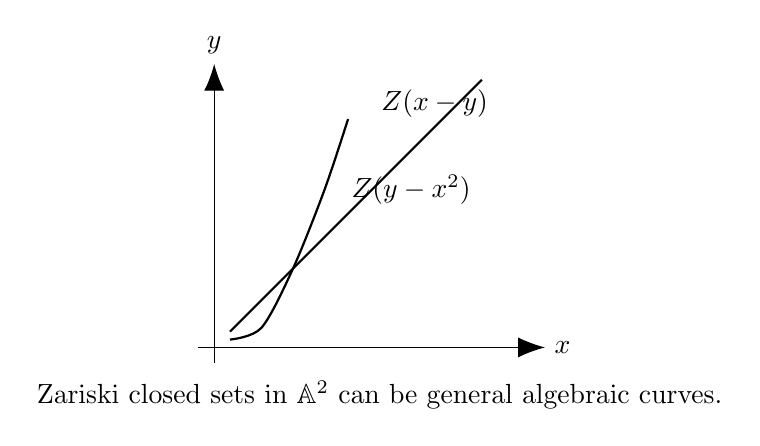
\begin{tikzpicture}[scale=1.0]
		\draw[->] (-0.2,0) -- (4.2,0) node[right] {$x$};
		\draw[->] (0,-0.2) -- (0,3.6) node[above] {$y$};
		
		% Zariski-closed curve: diagonal y=x
		\draw[thick] (0.2,0.2) -- (3.4,3.4);
		\node at (2.8,3.1) {$Z(x-y)$};
		
		% Another curve: parabola y=x^2 (schematic)
		\draw[thick] plot[smooth] coordinates {(0.2,0.1) (0.6,0.25) (1.0,1.0) (1.4,2.0) (1.7,2.9)};
		\node at (2.5,2.0) {$Z(y-x^2)$};
		
		\node at (2.1,-0.6) {Zariski closed sets in $\mathbb A^2$ can be general algebraic curves.};
	\end{tikzpicture}
	\caption{Zariski topology on $\mathbb A^2$: closed sets include diagonals and curves.}
\end{figure}

\begin{figure}[h]
	\centering
	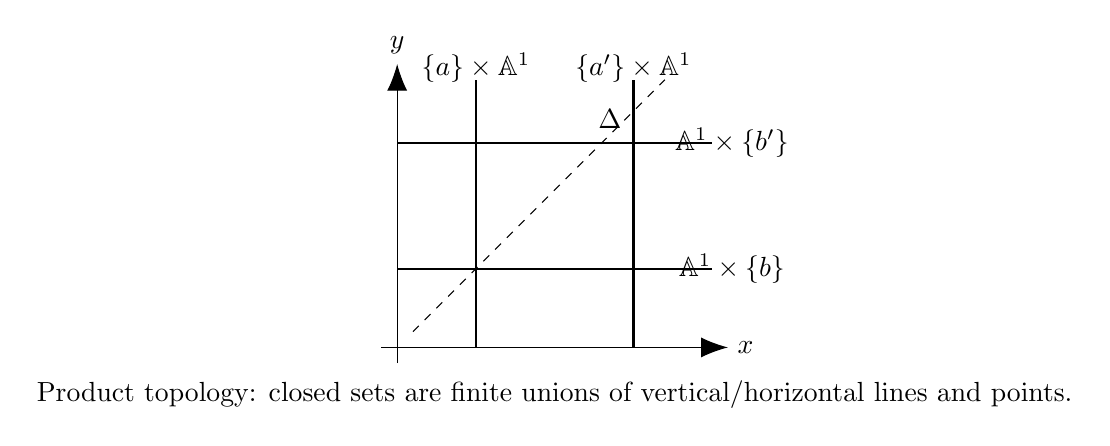
\begin{tikzpicture}[scale=1.0]
		\draw[->] (-0.2,0) -- (4.2,0) node[right] {$x$};
		\draw[->] (0,-0.2) -- (0,3.6) node[above] {$y$};
		
		% vertical lines (closed in product topology)
		\draw[thick] (1.0,0.0) -- (1.0,3.4);
		\draw[thick] (3.0,0.0) -- (3.0,3.4);
		\node at (1.0,3.55) {$\{a\}\times \mathbb A^1$};
		\node at (3.0,3.55) {$\{a'\}\times \mathbb A^1$};
		
		% horizontal lines (closed in product topology)
		\draw[thick] (0.0,1.0) -- (4.0,1.0);
		\draw[thick] (0.0,2.6) -- (4.0,2.6);
		\node at (4.25,1.0) {$\mathbb A^1\times\{b\}$};
		\node at (4.25,2.6) {$\mathbb A^1\times\{b'\}$};
		
		% diagonal (not closed in product topology) shown dashed
		\draw[dashed] (0.2,0.2) -- (3.4,3.4);
		\node at (2.7,2.9) {$\Delta$};
		
		\node at (2.0,-0.6) {Product topology: closed sets are finite unions of vertical/horizontal lines and points.};
	\end{tikzpicture}
	\caption{Product topology on $\mathbb A^1\times \mathbb A^1$ (each factor Zariski): the diagonal is not closed.}
\end{figure}

\subsection{More intuition: distinguished opens $D(f)$}

For $f\in k[x_1,\dots,x_n]$ define
\[
D(f)
=
\mathbb A^n\setminus Z(f).
\]
These sets are called \emph{distinguished opens} and they form a basis of the Zariski topology.

They satisfy the basic identities
\[
D(1)
=
\mathbb A^n,
\qquad
D(0)
=
\emptyset,
\]
\[
D(f)\cap D(g)
=
D(fg).
\]
In particular, finite intersections of distinguished opens are again distinguished opens.

Geometrically, $D(f)$ is obtained by removing the hypersurface $Z(f)$ from $\mathbb A^n$.
For example, in $\mathbb A^2$:
\[
D(x)
=
\mathbb A^2\setminus Z(x)
\quad
\text{(remove the $y$-axis)},
\]
\[
D(y)
=
\mathbb A^2\setminus Z(y)
\quad
\text{(remove the $x$-axis)},
\]
\[
D(xy)
=
D(x)\cap D(y)
=
\mathbb A^2\setminus (Z(x)\cup Z(y))
\quad
\text{(remove both axes)}.
\]

\subsection*{A Noetherian viewpoint and quasi-compactness}

A topological space is called \emph{Noetherian} if every descending chain of closed subsets stabilizes:
\[
F_1
\supset
F_2
\supset
F_3
\supset
\cdots
\quad
\Longrightarrow
\quad
F_N=F_{N+1}=F_{N+2}=\cdots
\text{ for some }N.
\]
Affine space $\mathbb A^n$ with the Zariski topology is Noetherian because the polynomial ring
\[
k[x_1,\dots,x_n]
\]
is Noetherian.

A fundamental consequence is that every Noetherian topological space is \emph{quasi-compact}:
every open cover admits a finite subcover.
Concretely, if
\[
X
=
\bigcup_{\alpha\in A} U_\alpha
\]
is an open cover of an affine variety $X$, then there exist finitely many indices
\[
\alpha_1,\dots,\alpha_r
\]
such that
\[
X
=
U_{\alpha_1}\cup\cdots\cup U_{\alpha_r}.
\]
This explains why Zariski-open sets are typically large and why finiteness phenomena occur frequently.

\begin{figure}[h]
	\centering
	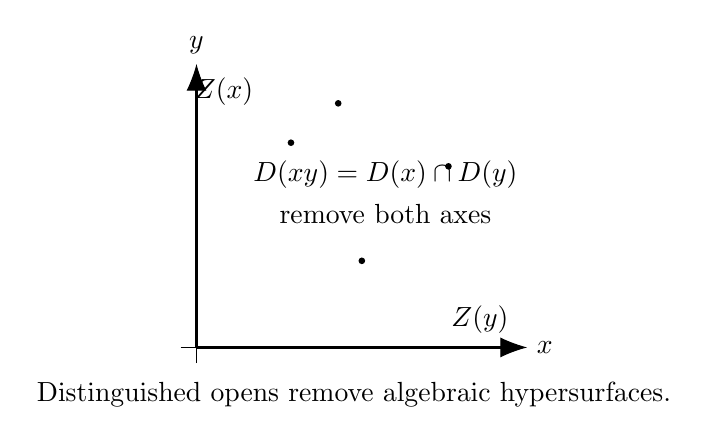
\begin{tikzpicture}[scale=1.0]
		\draw[->] (-0.2,0) -- (4.2,0) node[right] {$x$};
		\draw[->] (0,-0.2) -- (0,3.6) node[above] {$y$};
		
		% axes as closed sets Z(x) and Z(y)
		\draw[thick] (0,0) -- (0,3.4);
		\draw[thick] (0,0) -- (4.0,0);
		\node at (0.35,3.25) {$Z(x)$};
		\node at (3.6,0.35) {$Z(y)$};
		
		% indicate open region D(xy) = complement of union of axes
		\node at (2.4,2.2) {$D(xy)=D(x)\cap D(y)$};
		\node at (2.4,1.7) {remove both axes};
		
		% a few points to suggest "most points remain"
		\fill (1.2,2.6) circle (1.2pt);
		\fill (2.1,1.1) circle (1.2pt);
		\fill (3.2,2.3) circle (1.2pt);
		\fill (1.8,3.1) circle (1.2pt);
		
		\node at (2.0,-0.6) {Distinguished opens remove algebraic hypersurfaces.};
	\end{tikzpicture}
	\caption{Example in $\mathbb A^2$: $D(xy)$ is the complement of $Z(x)\cup Z(y)$.}
\end{figure}


\subsection*{Examples over an algebraically closed field}

Assume that $k$ is algebraically closed.

\subsubsection*{Examples in $\mathbb A^1$}

Let $t$ be the coordinate on $\mathbb A^1$.

\begin{enumerate}
	\item \textbf{Closed sets.}
	The Zariski-closed subsets of $\mathbb A^1$ are exactly
	\[
	\emptyset,
	\quad
	\text{finite subsets of }k,
	\quad
	\mathbb A^1.
	\]
	Indeed, for $f\in k[t]$ with $f\neq 0$,
	\[
	Z(f)
	=
	\{t\in k\mid f(t)=0\}
	\]
	is finite, and every finite set is
	\[
	\{a_1,\dots,a_r\}
	=
	Z\bigl((t-a_1)\cdots(t-a_r)\bigr).
	\]
	
	\item \textbf{Open sets.}
	The nonempty open subsets are exactly complements of finite sets:
	\[
	\mathbb A^1\setminus \{a_1,\dots,a_r\}.
	\]
	In particular, every nonempty open subset is dense.
	
	\item \textbf{Distinguished opens.}
	For $f\in k[t]$,
	\[
	D(f)=\mathbb A^1\setminus Z(f).
	\]
	For example,
	\[
	D(t)
	=
	\mathbb A^1\setminus\{0\},
	\qquad
	D(t(t-1))
	=
	\mathbb A^1\setminus\{0,1\}.
	\]
\end{enumerate}

\subsubsection*{Examples in $\mathbb A^2$}

Write coordinates $(x,y)$ on $\mathbb A^2$.

\begin{enumerate}
	\item \textbf{Lines.}
	A line is Zariski closed, for example
	\[
	Z(y)
	\quad
	\text{(the $x$-axis)},
	\qquad
	Z(x)
	\quad
	\text{(the $y$-axis)},
	\qquad
	Z(x-y)
	\quad
	\text{(the diagonal)}.
	\]
	
	\item \textbf{Unions via products.}
	For polynomials $f,g$,
	\[
	Z(fg)
	=
	Z(f)\cup Z(g).
	\]
	Example:
	\[
	Z(xy)
	=
	Z(x)\cup Z(y),
	\]
	the union of the two coordinate axes.
	
	\item \textbf{Parabola and hyperbola.}
	Examples of irreducible plane curves:
	\[
	Z(y-x^2),
	\qquad
	Z(xy-1).
	\]
	
	\item \textbf{Finite sets of points.}
	A point $(a,b)$ is Zariski closed:
	\[
	\{(a,b)\}
	=
	Z(x-a,\;y-b).
	\]
	Any finite set is a finite union of such points, hence closed.
	
	\item \textbf{A curve with isolated points.}
	If $f$ factors, a closed set can be a union of components of different dimensions.
	Example:
	\[
	Z\bigl(y(xy-1)\bigr)
	=
	Z(y)\cup Z(xy-1),
	\]
	a line together with a hyperbola.
	
	\item \textbf{Distinguished opens.}
	Typical opens:
	\[
	D(x)
	=
	\mathbb A^2\setminus Z(x),
	\qquad
	D(y)
	=
	\mathbb A^2\setminus Z(y),
	\]
	\[
	D(xy)
	=
	D(x)\cap D(y)
	=
	\mathbb A^2\setminus (Z(x)\cup Z(y)).
	\]
	More generally,
	\[
	D(f)\cap D(g)=D(fg).
	\]
\end{enumerate}

\subsubsection*{Examples contrasting $\mathbb A^2$ (Zariski) and $\mathbb A^1\times \mathbb A^1$ (product topology)}

Equip each factor $\mathbb A^1$ with the Zariski topology, and give $\mathbb A^1\times \mathbb A^1$ the product topology.

\begin{enumerate}
	\item \textbf{Vertical and horizontal lines are closed in the product topology.}
	For $a,b\in k$,
	\[
	\{a\}\times \mathbb A^1,
	\qquad
	\mathbb A^1\times \{b\}
	\]
	are closed, because $\{a\}$ and $\{b\}$ are closed in $\mathbb A^1$.
	
	\item \textbf{Finite unions of such lines and points are closed.}
	For example,
	\[
	\bigl(\{0\}\times \mathbb A^1\bigr)
	\cup
	\bigl(\mathbb A^1\times\{1\}\bigr)
	\cup
	\{(2,3)\}
	\]
	is closed in the product topology.
	
	\item \textbf{The diagonal is closed in Zariski on $\mathbb A^2$, but not closed in the product topology.}
	In $\mathbb A^2$ with coordinates $(x,y)$,
	\[
	\Delta
	=
	\{(t,t)\mid t\in k\}
	=
	Z(x-y),
	\]
	so $\Delta$ is Zariski closed.
	
	In the product topology on $\mathbb A^1\times \mathbb A^1$, closed sets are generated by rectangles
	\[
	C\times D
	\]
	with $C,D$ finite or all of $\mathbb A^1$.
	In particular, one can show that every closed set is a finite union of vertical lines, horizontal lines, and points.
	The diagonal $\Delta$ is not of this form, hence it is not closed in the product topology.
\end{enumerate}

\subsection*{Comparison table: Zariski on $\mathbb A^2$ vs product topology on $\mathbb A^1\times \mathbb A^1$}

Assume $k$ is algebraically closed.
We compare the Zariski topology on $\mathbb A^2$ with the product topology on
\[
\mathbb A^1\times \mathbb A^1
\]
when each factor carries the Zariski topology.

\begin{center}
	\renewcommand{\arraystretch}{1.3}
	\begin{tabular}{|p{0.27\textwidth}|p{0.34\textwidth}|p{0.34\textwidth}|}
		\hline
		\textbf{Topic}
		&
		\textbf{$\mathbb A^2$ with Zariski topology}
		&
		\textbf{$\mathbb A^1\times \mathbb A^1$ with product topology}
		\\
		\hline
		Closed sets
		&
		Sets of the form
		\[
		Z(I)
		\]
		for ideals $I\subset k[x,y]$.
		Geometrically: curves, finite unions of curves, finite sets of points, or combinations.
		&
		Finite unions of sets of the form
		\[
		\{a\}\times \mathbb A^1,
		\qquad
		\mathbb A^1\times \{b\},
		\]
		and finitely many points.
		\\
		\hline
		Basic open sets
		&
		Distinguished opens
		\[
		D(f)=\mathbb A^2\setminus Z(f),
		\quad
		f\in k[x,y].
		\]
		For example
		\[
		D(x),
		\qquad
		D(xy).
		\]
		&
		Products of cofinite opens:
		\[
		U\times V,
		\]
		where
		\[
		U=\mathbb A^1\setminus F,
		\qquad
		V=\mathbb A^1\setminus G,
		\]
		with $F,G$ finite.
		\\
		\hline
		Typical dense sets
		&
		Any nonempty open set is dense.
		For example
		\[
		D(f)
		\]
		is dense for $f\neq 0$.
		Curves are typically not dense.
		&
		Any nonempty open set (cofinite in each coordinate) is dense.
		A set missing only finitely many vertical and horizontal lines is dense.
		\\
		\hline
		Irreducible closed sets
		&
		Correspond to prime ideals in $k[x,y]$.
		Examples:
		\[
		Z(x-y),
		\qquad
		Z(y-x^2),
		\qquad
		Z(xy-1).
		\]
		&
		The irreducible closed sets are:
		\[
		\mathbb A^1\times \mathbb A^1,
		\quad
		\{a\}\times \mathbb A^1,
		\quad
		\mathbb A^1\times\{b\},
		\quad
		\{(a,b)\}.
		\]
		\\
		\hline
		Diagonal
		&
		Closed, because
		\[
		\Delta
		=
		Z(x-y).
		\]
		&
		Not closed.
		The closure of $\Delta$ is all of $\mathbb A^1\times \mathbb A^1$.
		\\
		\hline
		Key intuition
		&
		Closed sets can be defined by polynomial relations between coordinates.
		&
		Topology only sees finite exceptions in each coordinate separately,
		so relations like $x=y$ are not detected as closed.
		\\
		\hline
	\end{tabular}
\end{center}


\clearpage

\section*{Problem 2 — Nonempty opens in irreducible sets}

\textbf{Exact statement.}
Show that any non-empty open subset of an irreducible algebraic set is dense and irreducible.

\textbf{Solution.}
Let $X$ be irreducible and let $U\subset X$ be a nonempty open subset.

\emph{Density.}
Assume that $\overline{U}\neq X$.
Then
\[
X\setminus \overline{U}
\]
is a nonempty open subset of $X$, and it is disjoint from $U$.
This contradicts irreducibility (equivalently, in an irreducible space any two nonempty opens intersect).
Hence
\[
\overline{U}=X,
\]
so $U$ is dense in $X$.

\emph{Irreducibility.}
Suppose
\[
U
=
A\cup B,
\]
where $A,B$ are closed in the subspace topology on $U$.
Then there exist closed sets $F,G\subset X$ such that
\[
A
=
U\cap F,
\qquad
B
=
U\cap G.
\]
Taking closures in $X$ gives
\[
X
=
\overline{U}
\subset
F\cup G.
\]
Since $X$ is irreducible, we must have $X\subset F$ or $X\subset G$,
hence $U\subset F$ or $U\subset G$,
so $A=U$ or $B=U$.
Therefore $U$ is irreducible.

\subsection*{Algebraic sets versus affine varieties}

Assume that $k$ is algebraically closed.

\paragraph{Affine algebraic sets.}
A subset $X\subset \mathbb A^n$ is called an \emph{affine algebraic set} if there exists a set of polynomials
\[
S\subset k[x_1,\dots,x_n]
\]
such that
\[
X
=
Z(S)
=
\{\,p\in \mathbb A^n \mid f(p)=0 \text{ for all } f\in S\,\}.
\]
Equivalently, $X=Z(I)$ for some ideal $I\subset k[x_1,\dots,x_n]$.
Affine algebraic sets may be \emph{reducible}, meaning they can be written as a union of two proper closed subsets.

\paragraph{Affine varieties.}
An affine algebraic set $X$ is called an \emph{affine variety} if it is \emph{irreducible} in the Zariski topology.
Equivalently,
\[
X \text{ is an affine variety}
\quad\Longleftrightarrow\quad
I(X) \text{ is a prime ideal}
\quad\Longleftrightarrow\quad
A(X)=k[x_1,\dots,x_n]/I(X) \text{ is an integral domain}.
\]

\paragraph{Irreducible decomposition.}
Every affine algebraic set $X$ admits a finite decomposition into irreducible components:
\[
X
=
X_1\cup\cdots\cup X_r,
\]
where each $X_i$ is an affine variety and no $X_i$ is contained in another.
This decomposition is unique up to reordering.

\paragraph{Examples.}
In $\mathbb A^2$,
\[
Z(xy)
=
Z(x)\cup Z(y),
\]
so $Z(xy)$ is an algebraic set but not an affine variety.
By contrast,
\[
Z(y-x^2)
\]
is an affine variety because $y-x^2$ is irreducible.
A finite set of points is an affine algebraic set; it is an affine variety if and only if it consists of exactly one point.
Finally,
\[
\mathbb A^n
\]
is an affine variety since $I(\mathbb A^n)=(0)$ is prime.


\subsection*{Affine space, affine algebraic sets, and affine varieties}

Assume that $k$ is algebraically closed.

\paragraph{Affine space.}
Affine $n$-space over $k$ is
\[
\mathbb A^n_k
=
k^n
\]
equipped with coordinate functions $x_1,\dots,x_n$.
Its coordinate ring is
\[
k[\mathbb A^n]
=
k[x_1,\dots,x_n].
\]

\paragraph{Affine algebraic sets (algebraic sets).}
A subset $X\subset \mathbb A^n$ is called an \emph{affine algebraic set} if there exists a set of polynomials
\[
S\subset k[x_1,\dots,x_n]
\]
such that
\[
X
=
Z(S)
=
\{\,p\in \mathbb A^n \mid f(p)=0 \text{ for all } f\in S\,\}.
\]
Equivalently, $X=Z(I)$ for some ideal $I\subset k[x_1,\dots,x_n]$.
Thus affine algebraic sets are exactly the Zariski closed subsets of $\mathbb A^n$.

\paragraph{Vanishing ideal and coordinate ring.}
For any subset $X\subset \mathbb A^n$ define the vanishing ideal
\[
I(X)
=
\{\,f\in k[x_1,\dots,x_n]\mid f(p)=0 \text{ for all } p\in X\,\}.
\]
If $X$ is an affine algebraic set, its coordinate ring is
\[
A(X)
=
k[x_1,\dots,x_n]/I(X).
\]

\paragraph{Affine varieties.}
An affine algebraic set $X$ is called an \emph{affine variety} if it is \emph{irreducible} in the Zariski topology.
Equivalently,
\[
X \text{ is an affine variety}
\quad\Longleftrightarrow\quad
I(X) \text{ is a prime ideal}
\quad\Longleftrightarrow\quad
A(X) \text{ is an integral domain}.
\]

\paragraph{Examples.}
In $\mathbb A^2$,
\[
Z(xy)
=
Z(x)\cup Z(y),
\]
so $Z(xy)$ is an affine algebraic set but not an affine variety.
By contrast,
\[
Z(y-x^2)
\]
is an affine variety.
A finite set of points is an affine algebraic set; it is an affine variety if and only if it consists of one point.


\section*{Theory for Problem 2: Irreducibility and dense open subsets}

\subsection*{Irreducible topological spaces}

A topological space $X$ is called \emph{irreducible} if it cannot be written as a union of two proper closed subsets.
Equivalently, there do not exist closed sets $F,G\subsetneq X$ such that
\[
X=F\cup G.
\]

There are several equivalent characterizations:

\begin{enumerate}
	\item $X$ is irreducible.
	\item Any two nonempty open subsets of $X$ intersect.
	\item Every nonempty open subset of $X$ is dense in $X$.
	\item If $X=F\cup G$ with $F,G$ closed, then $X=F$ or $X=G$.
\end{enumerate}

A subset $U\subset X$ is called \emph{dense} if
\[
\overline{U}=X.
\]

\subsection*{Irreducibility in affine algebraic geometry}

Let $X\subset \mathbb A^n$ be an affine algebraic set, and let $I(X)\subset k[x_1,\dots,x_n]$ be its vanishing ideal.
The coordinate ring is
\[
A(X)
=
k[x_1,\dots,x_n]/I(X).
\]
Then
\[
X \text{ is irreducible}
\quad\Longleftrightarrow\quad
I(X) \text{ is a prime ideal}
\quad\Longleftrightarrow\quad
A(X) \text{ is an integral domain}.
\]

\subsection*{Nonempty opens are dense and irreducible}

Let $X$ be an irreducible topological space and let $U\subset X$ be a nonempty open subset.

\paragraph{Density.}
If $\overline{U}\neq X$, then
\[
X\setminus \overline{U}
\]
is a nonempty open set disjoint from $U$, contradicting irreducibility.
Hence
\[
\overline{U}=X,
\]
so $U$ is dense.

\paragraph{Irreducibility.}
If $U=A\cup B$ with $A,B$ closed in $U$, then there exist closed sets $F,G\subset X$ such that
\[
A=U\cap F,
\qquad
B=U\cap G.
\]
Taking closures in $X$ yields
\[
X=\overline{U}\subset F\cup G.
\]
Since $X$ is irreducible, $X\subset F$ or $X\subset G$, hence $U\subset F$ or $U\subset G$, so $A=U$ or $B=U$.
Therefore $U$ is irreducible.

\subsection*{Examples}

Assume $k$ is algebraically closed.

\begin{enumerate}
	\item $\mathbb A^n$ is irreducible, since
	\[
	I(\mathbb A^n)=(0)
	\]
	is prime in the domain $k[x_1,\dots,x_n]$.
	
	\item A hypersurface $Z(f)\subset \mathbb A^n$ is irreducible if and only if $f$ is irreducible in $k[x_1,\dots,x_n]$.
	For example,
	\[
	Z(y-x^2)
	\]
	is irreducible, but
	\[
	Z(xy)
	=
	Z(x)\cup Z(y)
	\]
	is reducible.
	
	\item If $X$ is irreducible and $p\in X$ is a point, then
	\[
	X\setminus\{p\}
	\]
	is open and dense in $X$ (and still irreducible).
\end{enumerate}


\section*{Problem 3 — Distinguished opens form a basis}

\textbf{Exact statement.}
Recall that a collection of open sets $\mathcal B\subset \tau$ in a topology $\tau$
is a basis for $\tau$ if every open set in $\tau$ is a union of elements of $\mathcal B$.
Show that if $X$ is an affine variety, the collection of distinguished open sets
\[
\{\,D(f):=X\setminus Z(f)\mid f\in A(X)\,\}
\]
forms a basis for the Zariski topology on $X$.

\textbf{Solution.}
Let $U\subset X$ be Zariski open.
Then $X\setminus U$ is Zariski closed, so there exists an ideal $I\subset A(X)$ with
\[
X\setminus U
=
Z(I).
\]
Therefore
\[
U
=
X\setminus Z(I)
=
\{\,x\in X \mid \exists f\in I \text{ such that } f(x)\neq 0\,\}.
\]
Equivalently,
\[
U
=
\bigcup_{f\in I}
\{\,x\in X \mid f(x)\neq 0\,\}
=
\bigcup_{f\in I}
D(f).
\]
Hence every open set is a union of distinguished opens, so the sets $D(f)$ form a basis.

\section*{Theory for Problem 3: Distinguished open sets form a basis}

\subsection*{Bases of topologies}

Let $X$ be a topological space with topology $\tau$.
A collection $\mathcal B\subset \tau$ is called a \emph{basis} for $\tau$ if every open set $U\in \tau$ can be written as a union of elements of $\mathcal B$.

Equivalently, $\mathcal B$ is a basis if:
\begin{enumerate}
	\item For every $x\in X$ there exists $B\in \mathcal B$ such that $x\in B$.
	\item If $x\in B_1\cap B_2$ with $B_1,B_2\in \mathcal B$, then there exists $B_3\in \mathcal B$ such that
	\[
	x\in B_3\subset B_1\cap B_2.
	\]
\end{enumerate}

\subsection*{Distinguished opens}

Let $X$ be an affine variety with coordinate ring $A(X)$.
For $f\in A(X)$ define
\[
D_X(f)
=
\{\,x\in X\mid f(x)\neq 0\,\}
=
X\setminus Z_X(f).
\]
These sets are called \emph{distinguished opens}.

They satisfy
\[
D_X(1)=X,
\qquad
D_X(0)=\emptyset,
\]
and
\[
D_X(f)\cap D_X(g)=D_X(fg).
\]
In particular, finite intersections of distinguished opens are again distinguished opens.

\subsection*{Distinguished opens generate all Zariski opens}

Let $I\subset A(X)$ be an ideal and consider the closed set $Z_X(I)$.
Its complement is
\[
X\setminus Z_X(I)
=
\{\,x\in X \mid \exists f\in I \text{ with } f(x)\neq 0\,\}.
\]
Therefore
\[
X\setminus Z_X(I)
=
\bigcup_{f\in I} D_X(f).
\]
Since every Zariski open subset of $X$ is the complement of some $Z_X(I)$, it follows that every open subset of $X$ is a union of distinguished opens.
Hence the sets $D_X(f)$ form a basis of the Zariski topology on $X$.

\subsection*{Examples}

Assume $k$ is algebraically closed.

\begin{enumerate}
	\item In $\mathbb A^2$,
	\[
	D(x)
	=
	\mathbb A^2\setminus Z(x)
	\]
	is the plane with the $y$-axis removed, and
	\[
	D(xy)=D(x)\cap D(y)
	\]
	is the plane with both axes removed.
	
	\item Let $C=Z(y-x^2)\subset \mathbb A^2$. Then
	\[
	D_C(x)=C\setminus\{(0,0)\}.
	\]
	
	\item Let $X=Z(xy-1)\subset \mathbb A^2$. In $A(X)$ we have $xy=1$, so $x$ is invertible on $X$ and therefore
	\[
	D_X(x)=X.
	\]
\end{enumerate}

\subsection*{Affine algebraic sets and affine varieties}

Assume that $k$ is algebraically closed.

\paragraph{Affine algebraic sets.}
A subset $X\subset \mathbb A^n$ is called an \emph{affine algebraic set} if there exists a set of polynomials
\[
S\subset k[x_1,\dots,x_n]
\]
such that
\[
X
=
Z(S)
=
\{\,p\in \mathbb A^n \mid f(p)=0 \text{ for all } f\in S\,\}.
\]
Equivalently, there exists an ideal $I\subset k[x_1,\dots,x_n]$ such that
\[
X
=
Z(I).
\]
By Hilbert's basis theorem, every ideal is finitely generated, so every affine algebraic set can be written as
\[
X
=
Z(f_1,\dots,f_r)
\]
for some polynomials $f_1,\dots,f_r$.

\paragraph{Vanishing ideal and coordinate ring.}
For any subset $X\subset \mathbb A^n$, define its vanishing ideal
\[
I(X)
=
\{\,f\in k[x_1,\dots,x_n]\mid f(p)=0 \text{ for all } p\in X\,\}.
\]
If $X$ is an affine algebraic set, its coordinate ring is
\[
A(X)
=
k[x_1,\dots,x_n]/I(X).
\]

\paragraph{Affine varieties.}
An affine algebraic set $X$ is called an \emph{affine variety} if it is \emph{irreducible} in the Zariski topology.
Equivalently,
\[
X \text{ is an affine variety}
\quad\Longleftrightarrow\quad
I(X) \text{ is a prime ideal}
\quad\Longleftrightarrow\quad
A(X) \text{ is an integral domain}.
\]


\section*{Problem 4 — Uniqueness of irreducible decomposition}

\textbf{Exact statement.}
Let $X\subset \mathbb A^n$ be an affine variety.
Suppose
\[
X
=
X_1\cup\cdots\cup X_r
\]
and
\[
X
=
X'_1\cup\cdots\cup X'_s
\]
are two decompositions of $X$ into irreducible components.
Assume that $X_i\not\subset X_j$ and $X'_i\not\subset X'_j$ for any $i\neq j$.
Prove that $r=s$ and that the two decompositions agree up to reordering.

\textbf{Solution.}
Fix $i$.
Since
\[
X_i
\subset
\bigcup_{j=1}^s
X'_j,
\]
and $X_i$ is irreducible, it follows that $X_i$ is contained in a single $X'_{j(i)}$.
Thus
\[
X_i
\subset
X'_{j(i)}.
\]
But $X_i$ is an irreducible component, i.e.\ a maximal irreducible subset of $X$.
Hence the inclusion forces
\[
X_i
=
X'_{j(i)}.
\]
Therefore the map $i\mapsto j(i)$ is injective, so
\[
r\le s.
\]
By symmetry (swapping the roles of $X_i$ and $X'_j$) we also get
\[
s\le r.
\]
Hence
\[
r=s,
\]
and after reindexing, the collections $\{X_1,\dots,X_r\}$ and $\{X'_1,\dots,X'_r\}$ coincide.

\section*{Theory for Problem 4: Irreducible components and uniqueness of decomposition}

\subsection*{Irreducible components in Noetherian spaces}

Assume that $k$ is algebraically closed.
Affine algebraic sets are Noetherian topological spaces in the Zariski topology.
In any Noetherian topological space $X$, every closed subset can be written as a finite union of irreducible closed subsets:
\[
X
=
X_1\cup\cdots\cup X_r.
\]
Moreover, we may choose the $X_i$ to be \emph{irreducible components}, meaning that each $X_i$ is irreducible and maximal (with respect to inclusion) among irreducible closed subsets of $X$.

\subsection*{Existence of irreducible decomposition}

Let $X$ be a closed subset of a Noetherian topological space.
If $X$ is irreducible, we are done.
Otherwise, we can write
\[
X=F\cup G
\]
with $F,G$ proper closed subsets.
Applying the same step to $F$ and $G$ and using the descending chain condition for closed sets, this process terminates after finitely many steps and produces a finite union of irreducible closed sets.
Thus irreducible decompositions exist and are finite.

\subsection*{Uniqueness up to reordering}

Suppose
\[
X=X_1\cup\cdots\cup X_r
\]
and
\[
X=X'_1\cup\cdots\cup X'_s
\]
are decompositions into irreducible components, and assume there are no containments
\[
X_i\subset X_j,
\qquad
X'_i\subset X'_j
\]
for $i\neq j$.
Fix $i$.
Since
\[
X_i
\subset
\bigcup_{j=1}^s X'_j
\]
and $X_i$ is irreducible, we must have
\[
X_i\subset X'_{j(i)}
\]
for some $j(i)$.
By maximality of irreducible components, this forces
\[
X_i=X'_{j(i)}.
\]
Hence $i\mapsto j(i)$ is injective, so $r\le s$.
By symmetry, $s\le r$.
Therefore
\[
r=s,
\]
and after reordering, the two collections of components coincide.

\subsection*{Algebraic description via minimal primes}

Let $X=Z(I)\subset \mathbb A^n$.
Then irreducible components correspond to the minimal prime ideals over $\sqrt I$:
\[
\sqrt I
=
\mathfrak p_1\cap\cdots\cap \mathfrak p_r,
\]
with each $\mathfrak p_i$ prime and minimal over $\sqrt I$.
Geometrically this yields
\[
X
=
Z(\mathfrak p_1)\cup\cdots\cup Z(\mathfrak p_r),
\]
and the sets $Z(\mathfrak p_i)$ are exactly the irreducible components.

\subsection*{Examples}

\begin{enumerate}
	\item In $\mathbb A^2$,
	\[
	Z(xy)=Z(x)\cup Z(y),
	\]
	so the irreducible components are the two coordinate axes.
	
	\item In $\mathbb A^2$,
	\[
	Z\bigl(y(y-x^2)\bigr)
	=
	Z(y)\cup Z(y-x^2),
	\]
	a line together with a parabola.
	
	\item In $\mathbb A^3$,
	\[
	Z(xz,yz)
	=
	Z(z)\cup Z(x,y),
	\]
	a plane together with a line.
\end{enumerate}

\begin{figure}[h]
	\centering
	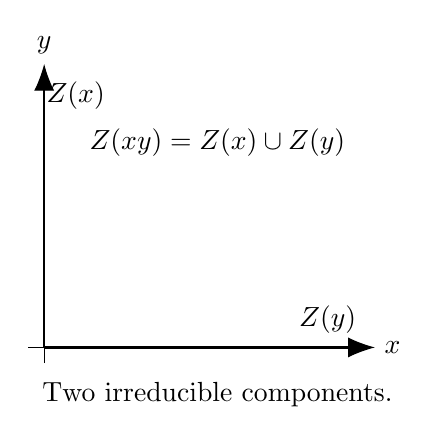
\begin{tikzpicture}[scale=1.0]
		\draw[->] (-0.2,0) -- (4.2,0) node[right] {$x$};
		\draw[->] (0,-0.2) -- (0,3.6) node[above] {$y$};
		
		% axes: Z(xy)=Z(x) U Z(y)
		\draw[thick] (0,0) -- (0,3.4);
		\draw[thick] (0,0) -- (4.0,0);
		\node at (0.4,3.2) {$Z(x)$};
		\node at (3.6,0.35) {$Z(y)$};
		
		\node at (2.2,2.6) {$Z(xy)=Z(x)\cup Z(y)$};
		\node at (2.2,-0.6) {Two irreducible components.};
	\end{tikzpicture}
	\caption{Reducible curve decomposes into irreducible components.}
\end{figure}


\section*{Problem 5 — Density of invertible / full-rank matrices}

\textbf{Exact statement.}
Identify $\mathbb A^{mn}_{\mathbb C}$ with the set of complex $m\times n$ matrices.
Prove that the subset $GL_n(\mathbb C)$ of invertible matrices is Zariski dense in $\mathbb A^{n^2}$.
An $m\times n$ matrix is said to have full rank if it has a $k\times k$ minor of non-vanishing determinant,
where
\[
k
=
\min\{m,n\}.
\]
Show that the set of matrices of full rank is Zariski dense in $\mathbb A^{mn}$.

\textbf{Solution.}
On $\mathbb A^{n^2}$ (entries as coordinates), the determinant is a polynomial function
\[
\det
\in
\mathbb C[\text{entries}].
\]
Hence
\[
GL_n(\mathbb C)
=
\{A \mid \det(A)\neq 0\}
=
D(\det)
=
\mathbb A^{n^2}\setminus Z(\det).
\]
Since $Z(\det)$ is a proper closed subset, $D(\det)$ is a nonempty Zariski-open subset,
hence dense in the irreducible variety $\mathbb A^{n^2}$.

For $m\times n$ matrices, let $k=\min\{m,n\}$.
For each $k\times k$ minor $M$, its determinant is a polynomial
\[
\det(M)
\in
\mathbb C[\text{entries}].
\]
The set of full rank matrices is
\[
\bigcup_{M}
D(\det(M)).
\]
This is a Zariski-open subset of $\mathbb A^{mn}$, and it is nonempty.
Therefore it is dense in $\mathbb A^{mn}$.

\section*{Theory for Problem 5: Determinants, rank conditions, and Zariski density}

\subsection*{Non-vanishing conditions define Zariski opens}

In the Zariski topology, a basic open subset of an affine variety $X$ is a distinguished open set
\[
D_X(f)
=
\{\,x\in X\mid f(x)\neq 0\,\}.
\]
If $X$ is irreducible, then every nonempty open subset of $X$ is dense.

\subsection*{$GL_n$ is open and dense in $\mathbb A^{n^2}$}

Identify $\mathbb A^{n^2}$ with the affine space of $n\times n$ matrices with entries $(a_{ij})$.
The determinant
\[
\det
\in
k[a_{ij}]
\]
is a polynomial function.
The subset of invertible matrices is
\[
GL_n(k)
=
\{A\mid \det(A)\neq 0\}
=
D(\det)
=
\mathbb A^{n^2}\setminus Z(\det).
\]
Since $Z(\det)$ is a proper closed set and $GL_n(k)$ is nonempty (it contains the identity matrix), it follows that $GL_n(k)$ is a nonempty Zariski open subset.
Because $\mathbb A^{n^2}$ is irreducible, we conclude that $GL_n(k)$ is Zariski dense in $\mathbb A^{n^2}$.

\subsection*{Full rank matrices and minors}

Identify $\mathbb A^{mn}$ with the affine space of $m\times n$ matrices.
Let
\[
r
=
\min\{m,n\}.
\]
For each $r\times r$ minor $M$, the determinant
\[
\det(M)
\]
is a polynomial in the matrix entries.
A matrix has full rank if and only if at least one such minor is nonzero.
Therefore the full rank locus is
\[
\bigcup_{M} D(\det(M)),
\]
a Zariski open subset of $\mathbb A^{mn}$.
This set is nonempty (for example, a matrix containing an $r\times r$ identity block has full rank), hence it is dense in $\mathbb A^{mn}$.

\subsection*{Examples}

Assume $k$ is algebraically closed.

\begin{enumerate}
	\item For $n=1$,
	\[
	GL_1(k)=k^*
	=
	D(x)
	\subset \mathbb A^1,
	\]
	which is dense.
	
	\item For $n=2$, the singular locus is the hypersurface
	\[
	Z(ad-bc)
	\subset \mathbb A^4,
	\]
	so $GL_2(k)=D(ad-bc)$ is open and dense.
	
	\item For $2\times 3$ matrices, full rank means that at least one $2\times 2$ minor is nonzero, so the rank $\le 1$ locus is closed and the full rank locus is open and dense.
\end{enumerate}

\begin{figure}[h]
	\centering
	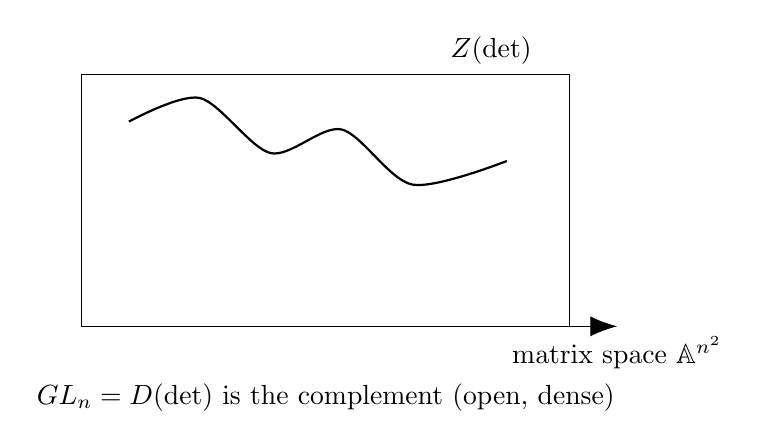
\begin{tikzpicture}[scale=1.0]
		% ambient "matrix space" rectangle (no text inside)
		\draw (0,0) rectangle (6.2,3.2);
		
		% a wavy curve representing the hypersurface Z(det)
		\draw[thick] plot[smooth] coordinates {(0.6,2.6) (1.5,2.9) (2.4,2.2) (3.3,2.5) (4.2,1.8) (5.4,2.1)};
		
		% axes arrow (to suggest ambient affine space)
		\draw[->] (0,0) -- (6.8,0);
		
		% labels outside the box
		\node at (5.2,3.5) {$Z(\det)$};
		\node[below] at (6.8,0) {matrix space $\mathbb A^{n^2}$};
		\node[below] at (3.1,-0.6) {$GL_n = D(\det)$ is the complement (open, dense)};
	\end{tikzpicture}
	\caption{Singular matrices form the hypersurface $Z(\det)$; invertible matrices are its open dense complement $D(\det)$.}
\end{figure}

\subsection*{Theory 5 — Implicit surfaces, regular points, tangent plane, and local graph charts}

A common representation of a surface in $\mathbb{R}^3$ is as a level set
\[
F(x,y,z)=0,
\]
where
\[
F:\mathbb{R}^3\to\mathbb{R}
\]
is at least $C^1$ (often $C^2$).

\paragraph{Regular points and smoothness.}
A point
\[
p=(x_0,y_0,z_0)
\]
with
\[
F(p)=0
\]
is called \emph{regular} if
\[
\nabla F(p)\neq 0.
\]
If $p$ is regular, then near $p$ the set $\{F=0\}$ is a smooth $2$-dimensional surface (a $2$-manifold embedded in $\mathbb{R}^3$).

\paragraph{Normal vector and tangent plane.}
At a regular point $p$, the gradient
\[
\nabla F(p)
\]
is normal to the surface. The tangent plane at $p$ is given by the linearization
\[
\nabla F(p)\cdot \bigl((x,y,z)-p\bigr)=0.
\]
Equivalently, writing
\[
\nabla F(p)=\bigl(F_x(p),F_y(p),F_z(p)\bigr),
\]
the tangent plane equation is
\[
F_x(p)(x-x_0)+F_y(p)(y-y_0)+F_z(p)(z-z_0)=0.
\]

\paragraph{Implicit Function Theorem (local graph form).}
If
\[
F_z(p)\neq 0,
\]
then there exists a neighborhood $U$ of $(x_0,y_0)$ and a $C^1$ function
\[
z=f(x,y)
\]
such that near $p$ the surface is exactly
\[
z=f(x,y),
\]
and this graph satisfies
\[
F\bigl(x,y,f(x,y)\bigr)=0.
\]
Similarly:
\[
F_x(p)\neq 0
\quad\Rightarrow\quad
x=g(y,z),
\]
\[
F_y(p)\neq 0
\quad\Rightarrow\quad
y=h(x,z).
\]
This is the basic mechanism behind building \emph{charts} (local coordinate patches) for an implicit surface.

\paragraph{Switching representations.}
Any explicit graph
\[
z=f(x,y)
\]
can be written implicitly by
\[
F(x,y,z)=z-f(x,y).
\]
However, a general implicit surface may fail to be a global graph (it can have overhangs or multiple sheets), so one typically uses multiple local charts (an atlas).

\paragraph{Singular points.}
If
\[
F(p)=0
\quad\text{and}\quad
\nabla F(p)=0,
\]
then $p$ is \emph{singular}. Near singularities, the level set may fail to be a smooth surface (it can self-intersect, have cusps, cones, etc.).

\section*{Problem 6 — Plane curves without common components; quasi-compactness}

\textbf{Exact statement.}
Let $f,g\in k[x,y]$ be polynomials which have no common factor.
Show that there exist $u,v\in k[x,y]$ such that $uf+vg$ is a non-zero polynomial in $k[x]$.
Now assume that $f$ is irreducible, and show that any proper subvariety of $Z(f)$ is finite
--- that is, affine plane curves which do not share a component intersect in finitely many points.
Deduce that $\mathbb A^2$ with the Zariski topology has the property that every open cover has a finite subcover.

\textbf{Solution.}
Since $f$ and $g$ have no common factor, their resultant with respect to $y$ satisfies
\[
R(x)
:=
\operatorname{Res}_y(f,g)
\in
k[x],
\qquad
R(x)\neq 0.
\]
A standard property of the resultant gives polynomials $u,v\in k[x,y]$ such that
\[
u f + v g
=
R(x),
\]
so in particular $u f + v g$ is a nonzero polynomial in $k[x]$.

Now assume $f$ is irreducible and let $W\subsetneq Z(f)$ be a proper subvariety.
Then $I(W)$ strictly contains $(f)$, so we can choose
\[
g\in I(W)\setminus (f).
\]
Since $f$ is irreducible, this implies
\[
\gcd(f,g)=1.
\]
Hence, by the first part, there exists
\[
R(x)\in k[x]\setminus\{0\}
\]
with
\[
R(x)\in (f,g).
\]
Therefore
\[
Z(f,g)
\subset
Z(R(x)).
\]
Since $Z(R(x))\subset \mathbb A^2$ consists of finitely many vertical lines
(and each vertical line meets $Z(f,g)$ in finitely many points),
it follows that
\[
Z(f,g)
\]
is finite.
Finally,
\[
W
\subset
Z(f)\cap Z(g)
=
Z(f,g),
\]
so $W$ is finite.

For the last claim, note that $k[x,y]$ is a Noetherian ring, so $\mathbb A^2$ is a Noetherian topological space
in the Zariski topology.
Every Noetherian topological space is quasi-compact, i.e.\ every open cover admits a finite subcover.

\section*{Theory 6 — Algebraic surfaces and comparison to implicit/explicit surfaces}

An \emph{algebraic surface} in $\mathbb{R}^3$ is a set of the form
\[
P(x,y,z)=0,
\]
where
\[
P\in\mathbb{R}[x,y,z]
\]
is a polynomial.

\paragraph{Key inclusion relations.}
Every algebraic surface is an implicit surface (polynomial level set):
\[
\{P=0\}\subset \{F=0\}\ \text{(with }F=P\text{)}.
\]
But not every implicit surface is algebraic, since $F$ may involve non-polynomial functions such as
\[
\sin,\ \exp,\ \log,\ \sqrt{\cdot}.
\]

\paragraph{Degree and complexity.}
The \emph{degree} of an algebraic surface is
\[
\deg(P).
\]
Higher degree typically allows more geometric/topological complexity (more components, more complicated intersections), though the exact behavior depends on the real locus.

\paragraph{Regular vs singular points (algebraic case).}
The same regularity test applies:
\[
\nabla P(p)\neq 0
\quad\Rightarrow\quad
\{P=0\}\ \text{is a smooth surface near }p.
\]
Singularities occur at points satisfying
\[
P(p)=0,
\]
\[
P_x(p)=0,
\]
\[
P_y(p)=0,
\]
\[
P_z(p)=0.
\]

\paragraph{Local graph charts for algebraic surfaces.}
If at a point $p$ on $\{P=0\}$ we have (for example)
\[
P_z(p)\neq 0,
\]
then by the Implicit Function Theorem there is a local representation
\[
z=f(x,y),
\]
even though $P$ is polynomial. Importantly, the resulting local $f$ need not be polynomial; it is generally just smooth (or analytic) locally.

\paragraph{Intersections and computational advantages.}
Algebraic surfaces have strong symbolic structure:
\begin{itemize}
	\item Intersections of algebraic surfaces reduce to solving polynomial systems.
	\item One can use elimination/resultants or Gröbner bases (in symbolic workflows).
	\item Many geometric queries (singular set, components, degree bounds) have algebraic formulations.
\end{itemize}

\paragraph{Comparison with general explicit graphs.}
If
\[
z=f(x,y)
\]
and $f$ is a polynomial, then the surface is algebraic because
\[
P(x,y,z)=f(x,y)-z
\]
is polynomial.
If $f$ is not polynomial (e.g.\ trigonometric/exponential), then the surface is generally not algebraic.

\paragraph{Practical viewpoint (modeling/visualization).}
\begin{itemize}
	\item \textbf{Explicit graphs} are easiest to sample but cannot represent multi-valued geometry globally.
	\item \textbf{Implicit surfaces} are most general and naturally handle multiple sheets.
	\item \textbf{Algebraic surfaces} are a structured subclass of implicit surfaces with strong symbolic tools, but can have unavoidable singularities and high-degree complexity.
\end{itemize}




\section*{Problem 7 — The hyperbola $xy=1$}

\textbf{Exact statement.}
Let $X\subset \mathbb A^2$ be the affine plane curve
\[
X
:=
Z(xy-1).
\]
Show that $X$ is not isomorphic to $\mathbb A^1$,
and describe all morphisms $\mathbb A^1\to X$.

\textbf{Solution.}
The coordinate ring is
\[
A(X)
=
k[x,y]/(xy-1).
\]
Since $xy=1$ in $A(X)$, we have $y=x^{-1}$, hence
\[
A(X)
\cong
k[x,x^{-1}],
\]
the Laurent polynomial ring.
This ring has nonconstant units, e.g.
\[
x^n
\]
for all $n\in \mathbb Z$.
By contrast,
\[
k[t]^\times
=
k^\times.
\]
Therefore $A(X)\not\cong k[t]$, so $X\not\cong \mathbb A^1$.

A morphism
\[
\varphi:\mathbb A^1\to X
\]
corresponds to a $k$-algebra map
\[
\varphi^*:
k[x,x^{-1}]
\to
k[t].
\]
The element $\varphi^*(x)$ must be a unit in $k[t]$, hence a constant
\[
\varphi^*(x)=c\in k^\times.
\]
Then
\[
\varphi^*(y)
=
\varphi^*(x^{-1})
=
c^{-1}.
\]
Thus every morphism $\mathbb A^1\to X$ is constant, of the form
\[
t
\longmapsto
(c,c^{-1}),
\qquad
c\in k^\times.
\]

\section*{Theory 7 — Affine curves, coordinate rings, and morphisms $\mathbb{A}^1 \to X$}

Fix a field $k$ (often assumed algebraically closed in basic affine algebraic geometry).
For an affine algebraic set
\[
X \subset \mathbb{A}^n,
\]
defined by an ideal
\[
I(X) \subset k[x_1,\dots,x_n],
\]
its coordinate ring is
\[
A(X)
=
k[x_1,\dots,x_n]/I(X).
\]

\paragraph{Morphisms via coordinate rings.}
For affine varieties (or affine algebraic sets), morphisms correspond contravariantly to $k$-algebra homomorphisms:
\[
\mathrm{Mor}(X,Y)
\ \cong\
\mathrm{Hom}_{k\text{-alg}}(A(Y),A(X)).
\]
In particular,
\[
A(\mathbb{A}^1)=k[t],
\]
so morphisms
\[
\mathbb{A}^1 \to X
\]
correspond to $k$-algebra maps
\[
A(X)\to k[t].
\]
Concretely, a morphism $\varphi:\mathbb{A}^1\to X\subset \mathbb{A}^n$ is given by polynomials
\[
x_i(t)\in k[t]
\]
such that the defining equations of $X$ vanish after substitution.

\paragraph{Isomorphisms of affine varieties.}
Two affine varieties $X,Y$ are isomorphic if and only if
\[
A(X)\cong A(Y)
\]
as $k$-algebras.

\paragraph{Units and the hyperbola $xy=1$.}
For
\[
X=Z(xy-1)\subset \mathbb{A}^2,
\]
the coordinate ring is
\[
A(X)
=
k[x,y]/(xy-1).
\]
In this ring,
\[
xy=1
\]
so $x$ is invertible with inverse $y$, hence
\[
A(X)\cong k[x,x^{-1}],
\]
the Laurent polynomial ring.
A key fact is that the units of $k[t]$ are exactly
\[
k[t]^\times = k^\times,
\]
so any $k$-algebra map
\[
k[x,x^{-1}] \to k[t]
\]
must send $x$ to a unit of $k[t]$, hence to a constant in $k^\times$.
This heavily restricts morphisms $\mathbb{A}^1\to X$.

\section*{Problem 8 — Components of $Z(x^2-yz,\;xz-x)$}

\textbf{Exact statement.}
Let
\[
Y
=
Z(x^2-yz,\;xz-x)
\subset
\mathbb A^3.
\]
Show that $Y$ has three irreducible components.
Describe the three components and their corresponding prime ideals.

\textbf{Solution.}
We rewrite the defining equations as
\[
x^2-yz
=
0,
\qquad
xz-x
=
x(z-1)
=
0.
\]
Hence for any point of $Y$ we have either
\[
z=1
\]
or
\[
x=0.
\]

If $z=1$, then $x^2-yz=0$ becomes
\[
x^2-y=0,
\]
so we obtain the irreducible curve
\[
C
=
Z(z-1,\;y-x^2).
\]
Its coordinate ring is isomorphic to $k[x]$, hence the ideal
\[
(z-1,\;y-x^2)
\]
is prime.

If $x=0$, then $x^2-yz=0$ becomes
\[
yz=0,
\]
so we obtain the union of two lines
\[
L_1
=
Z(x,y),
\qquad
L_2
=
Z(x,z).
\]
Both ideals
\[
(x,y),
\qquad
(x,z)
\]
are prime, since the corresponding quotients are $k[z]$ and $k[y]$.

Therefore
\[
Y
=
L_1\cup L_2\cup C,
\]
and these are three irreducible components with prime ideals
\[
(x,y),
\qquad
(x,z),
\qquad
(z-1,\;y-x^2).
\]

\section*{Theory 8 — Irreducible components, radicals, and prime ideals}

\paragraph{Irreducibility and prime ideals.}
An affine algebraic set $X$ is \emph{irreducible} if it cannot be written as a union of two proper closed subsets.
Over an algebraically closed field, the following are equivalent:
\[
X \ \text{is irreducible},
\]
\[
I(X)\ \text{is prime},
\]
\[
A(X)\ \text{is an integral domain}.
\]

\paragraph{Radicals and set-theoretic equality.}
By Hilbert's Nullstellensatz (over algebraically closed $k$),
\[
I(Z(J))=\sqrt{J}.
\]
Thus, for describing irreducible components (which are defined set-theoretically), it is natural to pass to radicals.

\paragraph{Decomposition into irreducible components.}
Any affine algebraic set $X$ can be written uniquely (up to ordering) as a finite union
\[
X = X_1 \cup \cdots \cup X_r
\]
where each $X_i$ is irreducible and $X_i \nsubseteq X_j$ for $i\neq j$.
On the ideal side, this corresponds to
\[
I(X)
=
I(X_1)\cap \cdots \cap I(X_r),
\]
where the ideals $I(X_i)$ are exactly the \emph{minimal prime ideals} over $I(X)$.

\paragraph{Practical method.}
Given an ideal $I\subset k[x_1,\dots,x_n]$:
\begin{itemize}
	\item compute $\sqrt{I}$ (or at least the minimal primes over $I$),
	\item each minimal prime $\mathfrak{p}$ gives an irreducible component
	\[
	Z(\mathfrak{p})\subset Z(I).
	\]
\end{itemize}



\section*{Problem 9 — Products of affine algebraic sets}

\textbf{Exact statement.}
Show that if $X\subset \mathbb A^m$, $Y\subset \mathbb A^n$ are affine algebraic sets,
then
\[
X\times Y
\subset
\mathbb A^m\times \mathbb A^n
=
\mathbb A^{m+n}
\]
is also an affine algebraic set.
(More difficult: the product of irreducible varieties is irreducible).

\textbf{Solution.}
Write
\[
X
=
Z(I)
\subset
\mathbb A^m,
\qquad
I\subset k[x_1,\dots,x_m],
\]
and
\[
Y
=
Z(J)
\subset
\mathbb A^n,
\qquad
J\subset k[y_1,\dots,y_n].
\]
In $\mathbb A^{m+n}$ with coordinates $(x_1,\dots,x_m,y_1,\dots,y_n)$,
consider the ideal
\[
K
=
I\cdot k[x_1,\dots,x_m,y_1,\dots,y_n]
+
J\cdot k[x_1,\dots,x_m,y_1,\dots,y_n].
\]
Then a point $(x,y)$ lies in $Z(K)$ if and only if
\[
f(x)=0 \text{ for all } f\in I
\]
and
\[
g(y)=0 \text{ for all } g\in J,
\]
which is equivalent to
\[
x\in X
\quad\text{and}\quad
y\in Y.
\]
Hence
\[
Z(K)
=
X\times Y,
\]
so $X\times Y$ is an affine algebraic set.

(For the harder part: one shows
\[
A(X\times Y)
\cong
A(X)\otimes_k A(Y),
\]
and over an algebraically closed field, if $A(X),A(Y)$ are domains, then the tensor product is a domain,
so $X\times Y$ is irreducible.)


\subsection*{Theory 9 — Products of affine algebraic sets}

Let
\[
X\subset \mathbb{A}^m,
\qquad
Y\subset \mathbb{A}^n
\]
be affine algebraic sets with ideals
\[
I(X)\subset k[x_1,\dots,x_m],
\qquad
I(Y)\subset k[y_1,\dots,y_n].
\]

\paragraph{Product is affine algebraic.}
Under the identification
\[
\mathbb{A}^m\times \mathbb{A}^n \cong \mathbb{A}^{m+n},
\]
the product
\[
X\times Y
\]
is cut out by the ideal
\[
I(X\times Y)
=
I(X)\cdot k[x,y]\ +\ I(Y)\cdot k[x,y]
\ \subset\
k[x_1,\dots,x_m,y_1,\dots,y_n].
\]
Equivalently, $X\times Y$ is defined by taking the defining equations of $X$ in the $x$-variables together with the defining equations of $Y$ in the $y$-variables.

\paragraph{Coordinate ring of a product.}
One has a natural isomorphism
\[
A(X\times Y)
\ \cong\
A(X)\otimes_k A(Y).
\]

\paragraph{Irreducibility of products (harder direction).}
If $X$ and $Y$ are irreducible, then $A(X)$ and $A(Y)$ are domains.
Under suitable hypotheses (e.g.\ $k$ algebraically closed and $X,Y$ varieties), one can show that
\[
A(X)\otimes_k A(Y)
\]
is again a domain, hence
\[
X\times Y
\]
is irreducible.
(This is the algebraic reflection of the geometric fact that a product of irreducible varieties remains irreducible.)


\subsection*{Theory 10 — Morphisms $\mathbb{A}^1 \to$ plane curves and the UFD trick}

Let $E\subset \mathbb{A}^2$ be an affine plane curve defined by one equation
\[
F(x,y)=0,
\]
so
\[
A(E)=k[x,y]/(F).
\]
A morphism
\[
\varphi:\mathbb{A}^1\to E
\]
corresponds to a $k$-algebra map
\[
\varphi^* : A(E) \to k[t].
\]
Writing
\[
\varphi^*(x)=x(t),
\qquad
\varphi^*(y)=y(t),
\]
this is exactly the condition that the defining relation holds in $k[t]$:
\[
F(x(t),y(t))=0.
\]

\paragraph{UFD input for $k[t]$.}
The ring
\[
k[t]
\]
is a unique factorization domain (UFD).
Two standard consequences used in curve-morphism problems are:
\begin{itemize}
	\item If a polynomial is a square in $k[t]$, then in its prime factorization every irreducible factor occurs with even exponent.
	\item If $a(t),b(t)\in k[t]$ are coprime and
	\[
	a(t)b(t)
	\]
	is a square in $k[t]$, then both $a(t)$ and $b(t)$ are squares up to units in $k^\times$.
\end{itemize}

\paragraph{Square-free factor arguments.}
When the curve equation factors as
\[
y^2 = g(x)
\]
with $g(x)$ having distinct linear factors (or at least being square-free), substitution gives
\[
y(t)^2 = g(x(t)).
\]
Then $g(x(t))$ must be a square in $k[t]$.
In a UFD, this often forces strong restrictions on $x(t)$ (frequently implying $x(t)$ is constant), hence the morphism is constant.

\paragraph{Philosophy.}
Morphisms $\mathbb{A}^1\to E$ correspond to polynomial parametrizations of the curve.
For many smooth cubic curves (elliptic-type behavior), the UFD + square-free factorization shows that non-constant polynomial parametrizations cannot exist, hence every morphism $\mathbb{A}^1\to E$ is constant.

\section*{Problem 10 — No non-constant maps $\mathbb A^1\to E$}

\textbf{Exact statement.}
Show that there are no non-constant morphisms from $\mathbb A^1$ to
\[
E
:=
Z(y^2-x^3+x)
\subset
\mathbb A^2.
\]
\emph{[Hint: consider the images of $x$ and $y$ under the induced map
	$A(E)\to A(\mathbb A^1)=k[t]$, and use the fact that $k[t]$ is a UFD.]}

\textbf{Solution.}
A morphism
\[
\varphi:\mathbb A^1\to E
\]
corresponds to a $k$-algebra homomorphism
\[
\varphi^*:
k[x,y]/(y^2-x^3+x)
\to
k[t].
\]
Set
\[
a
=
\varphi^*(x),
\qquad
b
=
\varphi^*(y).
\]
The defining equation of $E$ becomes
\[
b^2
=
a^3-a
=
a(a-1)(a+1).
\]

Assume $\operatorname{char}(k)\neq 2$.
Then
\[
\gcd(a,a-1)=1,
\qquad
\gcd(a,a+1)=1,
\qquad
\gcd(a-1,a+1)=1.
\]
Since $k[t]$ is a UFD and the product $a(a-1)(a+1)$ is a square, each of the three pairwise coprime factors
is a square up to a unit.
If $k$ is algebraically closed, every unit in $k[t]$ is a square in $k^\times$,
so we may write
\[
a
=
p^2,
\qquad
a-1
=
q^2
\]
for some $p,q\in k[t]$.
Subtracting gives
\[
p^2-q^2
=
1,
\]
hence
\[
(p-q)(p+q)
=
1.
\]
Thus $p-q$ and $p+q$ are units in $k[t]$, so $p$ and $q$ are constant.
Therefore $a$ is constant, and then $b^2=a(a-1)(a+1)$ is constant, so $b$ is constant as well.
Hence $\varphi$ is constant, and there are no non-constant morphisms $\mathbb A^1\to E$.


\section{Problem 11 — The monomial curve $(t^3,t^4,t^5)$ in $\mathbb A^3$}

\textbf{Exact statement.}
Let $X\subset \mathbb A^3$ be the set
\[
\{(t^3,t^4,t^5)\mid t\in k\}.
\]
Show that $X$ is an affine variety, and determine $I(X)$.
\[
\text{[Hint: $I(X)$ can be generated by three elements.]}
\]
Show that $I(X)$ cannot be generated by two elements.

\textbf{Solution.}
Consider the $k$-algebra homomorphism
\[
\varphi:k[x,y,z]\to k[t],
\qquad
\varphi(x)=t^3,
\qquad
\varphi(y)=t^4,
\qquad
\varphi(z)=t^5.
\]
Then
\[
I(X)=\ker(\varphi).
\]

Define
\[
f_1
=
y^2-xz,
\qquad
f_2
=
x^3-yz,
\qquad
f_3
=
z^2-x^2y.
\]
Each satisfies
\[
f_i(t^3,t^4,t^5)=0,
\]
so
\[
J:=(f_1,f_2,f_3)\subset I(X),
\]
and hence
\[
X\subset Z(J).
\]

We now show that
\[
Z(J)=X.
\]
Let $(a,b,c)\in Z(J)$.
Then
\[
b^2=ac,
\qquad
a^3=bc,
\qquad
c^2=a^2b.
\]
If
\[
a=0,
\]
then $b^2=0$ gives $b=0$, and then $c^2=0$ gives $c=0$, so $(a,b,c)=(0,0,0)\in X$.
If
\[
a\neq 0,
\]
define
\[
t:=\frac{b}{a}\in k.
\]
From $a^3=bc$ we get
\[
c=\frac{a^3}{b}=\frac{a^2}{t}.
\]
Substitute into $b^2=ac$:
\[
a^2t^2
=
a\cdot \frac{a^2}{t},
\]
so
\[
t^3=a.
\]
Then
\[
a=t^3,
\qquad
b=at=t^4,
\qquad
c=\frac{a^2}{t}=t^5,
\]
so $(a,b,c)\in X$. Therefore
\[
Z(J)\subset X,
\]
and hence
\[
Z(J)=X.
\]
In particular, $X$ is Zariski closed, hence an affine variety.

Next we show
\[
I(X)=J.
\]
Modulo $J$ we have the relations
\[
y^2=xz,
\qquad
yz=x^3,
\qquad
z^2=x^2y.
\]
Using these, any monomial $x^ay^bz^c$ can be reduced until it has no factor $y^2$, $yz$, or $z^2$,
because each replacement strictly decreases $b+c$:
\[
y^2\mapsto xz,
\qquad
yz\mapsto x^3,
\qquad
z^2\mapsto x^2y.
\]
Thus every class in $k[x,y,z]/J$ is a $k$-linear combination of
\[
x^n,
\qquad
x^ny,
\qquad
x^nz,
\qquad
n\ge 0.
\]
The induced map
\[
\bar\varphi:k[x,y,z]/J\to k[t]
\]
sends these basis candidates to
\[
t^{3n},
\qquad
t^{3n+4},
\qquad
t^{3n+5}.
\]
All these exponents are distinct, hence these monomials are $k$-linearly independent in $k[t]$.
Therefore $\bar\varphi$ is injective, so
\[
\ker(\varphi)=J,
\]
and hence
\[
I(X)
=
(y^2-xz,\;x^3-yz,\;z^2-x^2y).
\]

Finally, $I(X)$ cannot be generated by two elements.
Indeed, reducing modulo $(x,z)\cong k[y]$ gives
\[
f_1\mapsto y^2\neq 0,
\qquad
f_2\mapsto 0,
\qquad
f_3\mapsto 0,
\]
so $f_1\notin (f_2,f_3)$.
Reducing modulo $(y,z)\cong k[x]$ gives
\[
f_2\mapsto x^3\neq 0,
\qquad
f_1\mapsto 0,
\qquad
f_3\mapsto 0,
\]
so $f_2\notin (f_1,f_3)$.
Reducing modulo $(x,y)\cong k[z]$ gives
\[
f_3\mapsto z^2\neq 0,
\qquad
f_1\mapsto 0,
\qquad
f_2\mapsto 0,
\]
so $f_3\notin (f_1,f_2)$.
Thus all three generators are necessary.

\section*{Theory 11 — Monomial (parametrized) curves, toric ideals, and minimal generators}

Let
\[
\phi:\mathbb{A}^1 \longrightarrow \mathbb{A}^3
\]
be a morphism given by polynomials
\[
\phi(t)=(t^3,t^4,t^5).
\]
Write coordinates on $\mathbb{A}^3$ as
\[
(x,y,z).
\]
Then the coordinate ring map is
\[
\phi^* : k[x,y,z] \longrightarrow k[t],
\]
\[
\phi^*(x)=t^3,
\]
\[
\phi^*(y)=t^4,
\]
\[
\phi^*(z)=t^5.
\]

\paragraph{Defining ideal as a kernel.}
The ideal of the image set
\[
X=\{(t^3,t^4,t^5)\mid t\in k\}
\]
is
\[
I(X)=\ker(\phi^*).
\]
Hence $X$ is an affine algebraic set, and if $I(X)$ is prime then $X$ is an affine variety.

\paragraph{Semigroup ring viewpoint.}
The image subring is
\[
k[t^3,t^4,t^5]\subset k[t],
\]
and one has an isomorphism
\[
A(X)
=
k[x,y,z]/I(X)
\ \cong\
k[t^3,t^4,t^5].
\]
Since $k[t^3,t^4,t^5]$ is a subring of the domain $k[t]$, it is a domain.
Therefore
\[
I(X)\ \text{is prime},
\]
and $X$ is an affine variety (irreducible).

\paragraph{Binomials from integer relations.}
For monomial curves, $I(X)$ is generated by binomials coming from additive relations among exponents.
A relation
\[
a\cdot 3+b\cdot 4+c\cdot 5
=
a'\cdot 3+b'\cdot 4+c'\cdot 5
\]
yields the binomial
\[
x^{a}y^{b}z^{c}-x^{a'}y^{b'}z^{c'}
\in I(X).
\]
Typical small relations here are:
\[
2\cdot 4 = 3+5,
\]
\[
3\cdot 3 = 4+5,
\]
\[
2\cdot 3+4 = 2\cdot 5.
\]
They give the binomials
\[
y^2-xz,
\]
\[
x^3-yz,
\]
\[
x^2y-z^2.
\]

\paragraph{Height and the “two generators” obstruction.}
Since $X$ is a (nontrivial) curve in $\mathbb{A}^3$, one has
\[
\dim(A(X))=1,
\]
\[
\mathrm{ht}\bigl(I(X)\bigr)=3-1=2.
\]
If an ideal of height $2$ in a polynomial ring were generated by two elements, it would be a \emph{complete intersection}.
Thus to prove $I(X)$ cannot be generated by two elements, it is enough to show that $I(X)$ is \emph{not} a complete intersection.

\paragraph{Local minimal number of generators.}
Let
\[
\mathfrak m=(x,y,z)\subset k[x,y,z]
\]
and localize at $\mathfrak m$.
For an ideal $I$, the minimal number of generators of $I_{\mathfrak m}$ equals
\[
\mu(I_{\mathfrak m})
=
\dim_k\!\Bigl(I/ \mathfrak m I\Bigr).
\]
Therefore:
\[
\dim_k\!\Bigl(I(X)/\mathfrak m I(X)\Bigr)=3
\quad\Longrightarrow\quad
I(X)\ \text{cannot be generated by two elements}.
\]
(Here one uses that the three basic binomials above have independent images modulo $\mathfrak m I(X)$.)

\medskip

\section{Problem 12 — Intersecting fibers for $z\neq 0$, parallel fiber at $z=0$}

\textbf{Exact statement.}
Let $\pi:\mathbb A^3\to \mathbb A^1$ be the projection onto the third coordinate.
For each point $z\in\mathbb A^1$, the set-theoretic preimage $\pi^{-1}(z)$ is isomorphic to $\mathbb A^2$.
Construct a variety $X\subset \mathbb A^3$ with the property that if $z\neq 0$ then
$\pi^{-1}(z)\cap X$ is a union of two intersecting lines in $\pi^{-1}(z)$,
but $\pi^{-1}(0)\cap X$ is a union of two parallel lines in $\pi^{-1}(0)$.

\textbf{Solution.}
Let $(x,y,z)$ be coordinates on $\mathbb A^3$.
Define $X$ by
\[
X
=
Z\bigl(y\,(y-zx-1)\bigr).
\]
Equivalently, $X$ is the union of the two hypersurfaces
\[
y=0
\]
and
\[
y=zx+1.
\]

Fix $c\in k$.
Inside the fiber
\[
\pi^{-1}(c)
=
\{z=c\}
\cong
\mathbb A^2,
\]
we have
\[
\pi^{-1}(c)\cap X
=
Z\bigl(y\,(y-cx-1)\bigr)
=
Z(y)\cup Z(y-cx-1).
\]
Thus $\pi^{-1}(c)\cap X$ is the union of the two lines
\[
y=0
\]
and
\[
y=cx+1.
\]
If
\[
c\neq 0,
\]
these lines intersect at
\[
(x,y)=\left(-\frac{1}{c},0\right).
\]
If
\[
c=0,
\]
the lines become
\[
y=0
\]
and
\[
y=1,
\]
which are parallel in the plane $z=0$.
This $X$ satisfies the required property.

\section*{Theory 12 — Families over $\mathbb{A}^1$, fibers under projection, and degeneration of line configurations}

Consider the projection
\[
\pi:\mathbb{A}^3 \longrightarrow \mathbb{A}^1,
\]
\[
\pi(x,y,z)=z.
\]
For each
\[
c\in \mathbb{A}^1,
\]
the set-theoretic fiber is the affine plane
\[
\pi^{-1}(c)=\{(x,y,z)\mid z=c\}
\ \cong\
\mathbb{A}^2.
\]

\paragraph{Varieties over $\mathbb{A}^1$.}
A subset
\[
X\subset \mathbb{A}^3
\]
defined by polynomial equations
\[
F_1(x,y,z)=0,\dots,F_r(x,y,z)=0
\]
defines a family over $\mathbb{A}^1$ via $\pi|_X$.
The fiber over $c$ is
\[
X_c
=
X\cap \pi^{-1}(c),
\]
which is cut out inside the plane $z=c$ by
\[
F_1(x,y,c)=0,\dots,F_r(x,y,c)=0.
\]

\paragraph{Set-theoretic vs scheme-theoretic behavior.}
Even if all fibers are unions of lines, the \emph{incidence pattern} can change with $c$:
\begin{itemize}
	\item two lines can intersect for $c\neq 0$ but become parallel at $c=0$,
	\item the intersection point can “escape to infinity” as $c\to 0$ in affine coordinates.
\end{itemize}
This is a standard degeneration phenomenon in affine families.

\paragraph{Two-line fibers via a factorized equation.}
If a single equation factors as
\[
F(x,y,z)=L_1(x,y,z)\,L_2(x,y,z),
\]
then each fiber is (set-theoretically) the union of the two lines
\[
L_1(x,y,c)=0
\quad\text{and}\quad
L_2(x,y,c)=0
\]
inside the plane $z=c$.

\paragraph{Parallel vs intersecting lines.}
Two lines in a plane are parallel precisely when their defining linear equations have proportional direction vectors (same slope) but different constants.
In a family
\[
L_2(x,y,c)=0,
\]
the slope can depend on $c$, so one can arrange:
\[
c\neq 0
\ \Rightarrow\
\text{non-parallel (hence intersecting)},
\]
\[
c=0
\ \Rightarrow\
\text{parallel}.
\]
A typical mechanism is that the intersection point depends on $c$ like
\[
x=-\frac{1}{c},
\]
which is not defined at $c=0$, meaning the intersection disappears from the affine chart and the limit configuration becomes parallel.

\medskip

\section{Problem 13 — Unions of lines in $\mathbb A^3$ and $\mathbb A^2$ are not isomorphic}

\textbf{Exact statement.}
Let $V\subset \mathbb A^3$ be the union of the $x$, $y$, and $z$ axes.
Let $W\subset \mathbb A^2$ be the union of the $x$-axis, $y$-axis, and the line $x=y$.
Calculate generators for $I(V)$ and $I(W)$, and show that $V$ is not isomorphic to $W$.
\[
\text{[Hint: use $\mathfrak m_p/\mathfrak m_p^2$.]}
\]

\textbf{Solution.}
Let $(x,y,z)$ be coordinates on $\mathbb A^3$.
The three coordinate axes have ideals
\[
I(\text{$x$-axis})=(y,z),
\qquad
I(\text{$y$-axis})=(x,z),
\qquad
I(\text{$z$-axis})=(x,y).
\]
Hence
\[
I(V)
=
(y,z)\cap(x,z)\cap(x,y).
\]
We claim that
\[
I(V)
=
(xy,\;xz,\;yz).
\]
Indeed, each of $xy,xz,yz$ lies in all three ideals, so
\[
(xy,xz,yz)\subset I(V).
\]
Conversely, if $f\in (y,z)\cap(x,z)\cap(x,y)$, then every monomial term of $f$ must vanish when two coordinates are set to $0$,
so every monomial is divisible by at least two of the variables $x,y,z$.
Therefore $f$ is a $k[x,y,z]$-linear combination of $xy,xz,yz$, proving
\[
I(V)=(xy,xz,yz).
\]

Now let $(x,y)$ be coordinates on $\mathbb A^2$.
The three lines have ideals
\[
I(\{y=0\})=(y),
\qquad
I(\{x=0\})=(x),
\qquad
I(\{x=y\})=(x-y).
\]
Hence
\[
I(W)
=
(y)\cap(x)\cap(x-y).
\]
A polynomial vanishes on $y=0$ if and only if it is divisible by $y$, similarly for $x=0$ and $x=y$.
Thus it is divisible by all three factors, so
\[
I(W)=(x\,y\,(x-y)).
\]

To show $V\not\cong W$, we use the invariant
\[
\dim_k\bigl(\mathfrak m_p/\mathfrak m_p^2\bigr),
\]
which equals the dimension of the Zariski tangent space at $p$ and is preserved by isomorphisms.

For $V$, the coordinate ring is
\[
A(V)=k[x,y,z]/(xy,xz,yz).
\]
If $p\neq (0,0,0)$, then $p$ lies on exactly one axis and is a smooth point, so
\[
\dim_k(\mathfrak m_p/\mathfrak m_p^2)=1.
\]
At the origin, let
\[
\mathfrak m=(x,y,z)\subset A(V).
\]
Because
\[
xy=0,
\qquad
xz=0,
\qquad
yz=0
\]
in $A(V)$, the square $\mathfrak m^2$ is generated by
\[
x^2,
\qquad
y^2,
\qquad
z^2.
\]
Hence the classes of $x,y,z$ are linearly independent modulo $\mathfrak m^2$, so
\[
\dim_k(\mathfrak m/\mathfrak m^2)=3.
\]
Thus $V$ has a point (the origin) with tangent dimension $3$.

For $W$, the coordinate ring is
\[
A(W)=k[x,y]/(xy(x-y)).
\]
Away from the origin, each point lies on exactly one line, so
\[
\dim_k(\mathfrak m_p/\mathfrak m_p^2)=1.
\]
At the origin, the defining equation $xy(x-y)$ has no linear terms, so the tangent space is all of $\mathbb A^2$, hence
\[
\dim_k(\mathfrak m/\mathfrak m^2)=2.
\]
Therefore the possible values of $\dim_k(\mathfrak m_p/\mathfrak m_p^2)$ on $W$ are only $1$ and $2$,
whereas on $V$ we also get the value $3$.
Since isomorphisms preserve this dimension, it follows that
\[
V\not\cong W.
\]






\section*{Theory 13 — Unions of linear subvarieties, intersections of ideals, and the tangent-space invariant}

\paragraph{Ideals of unions.}
For affine algebraic sets
\[
X_1,\dots,X_r \subset \mathbb{A}^n,
\]
one has
\[
I\Bigl(\bigcup_{i=1}^r X_i\Bigr)
=
\bigcap_{i=1}^r I(X_i).
\]
In particular, for unions of lines, each $I(X_i)$ is generated by linear polynomials, and the union ideal is an intersection of such linear ideals.

\paragraph{Coordinate axes in $\mathbb{A}^3$.}
Let
\[
V \subset \mathbb{A}^3
\]
be the union of the $x$-, $y$-, and $z$-axes.
Then
\[
I(\text{$x$-axis})=(y,z),
\]
\[
I(\text{$y$-axis})=(x,z),
\]
\[
I(\text{$z$-axis})=(x,y),
\]
so
\[
I(V)=(y,z)\cap(x,z)\cap(x,y).
\]
A standard computation gives
\[
(y,z)\cap(x,z)\cap(x,y)
=
(xy,xz,yz).
\]

\paragraph{Local rings and Zariski tangent space.}
Let $X\subset \mathbb{A}^n$ be affine and
\[
p\in X.
\]
Let
\[
\mathcal{O}_{X,p}
\]
be the local ring, and
\[
\mathfrak m_p
\]
its maximal ideal.
Then
\[
\mathfrak m_p/\mathfrak m_p^2
\]
is a finite-dimensional $k$-vector space, and its dual identifies with the Zariski tangent space:
\[
T_pX
\ \cong\
\mathrm{Hom}_k(\mathfrak m_p/\mathfrak m_p^2,k).
\]
In particular,
\[
\dim_k(\mathfrak m_p/\mathfrak m_p^2)=\dim(T_pX).
\]

\paragraph{Isomorphism invariant.}
If
\[
X \cong Y
\]
as affine algebraic sets, then for corresponding points
\[
p\in X,
\qquad
q\in Y,
\]
there is an induced isomorphism of local rings, hence
\[
\dim_k(\mathfrak m_p/\mathfrak m_p^2)
=
\dim_k(\mathfrak m_q/\mathfrak m_q^2).
\]
Therefore the function
\[
p \longmapsto \dim_k(\mathfrak m_p/\mathfrak m_p^2)
\]
is a powerful invariant for distinguishing non-isomorphic reducible varieties.

\paragraph{Geometric meaning for unions of lines.}
At a smooth point on a single line component, one has
\[
\dim_k(\mathfrak m_p/\mathfrak m_p^2)=1.
\]
At a multiple intersection point, this dimension equals the dimension of the linear span of the tangent directions of the branches in the ambient space.
Thus:
\begin{itemize}
	\item three coordinate axes meeting at the origin in $\mathbb{A}^3$ have three independent directions, so the tangent space at the origin has dimension $3$,
	\item three lines through the origin inside $\mathbb{A}^2$ span only a $2$-dimensional tangent space.
\end{itemize}
This is exactly the type of local invariant used to show that two unions of lines are not isomorphic.


\subsection*{Lemma Toolbox — Computing $\dim_k(\mathfrak m_p/\mathfrak m_p^2)$ from equations}

\textbf{Lemma (Tangent space from Jacobian / linear parts).}
Let
\[
X=Z(f_1,\dots,f_r)\subset \mathbb{A}^n_k
\]
and let
\[
p\in X.
\]
Write coordinates on $\mathbb{A}^n$ as
\[
x_1,\dots,x_n.
\]
Let
\[
J(p)=\left(\frac{\partial f_i}{\partial x_j}(p)\right)_{1\le i\le r,\ 1\le j\le n}
\]
be the Jacobian matrix at $p$.
Then the Zariski tangent space satisfies
\[
T_pX
=
\ker\!\bigl(J(p):k^n\to k^r\bigr),
\]
hence
\[
\dim_k(T_pX)
=
n-\mathrm{rank}\,J(p).
\]
Moreover,
\[
\dim_k(\mathfrak m_p/\mathfrak m_p^2)
=
\dim_k(T_pX).
\]

\textbf{Equivalent formulation (linear parts).}
Translate so that $p=0$ (replace $x_j$ by $x_j-x_j(p)$).
Write each $f_i$ as
\[
f_i
=
\ell_i
+
\text{(terms of total degree $\ge 2$)},
\]
where $\ell_i$ is the linear part.
Then
\[
T_0X=Z(\ell_1,\dots,\ell_r)\subset k^n,
\]
so
\[
\dim_k(\mathfrak m_0/\mathfrak m_0^2)
=
n-\dim_k\langle \ell_1,\dots,\ell_r\rangle,
\]
where $\langle \ell_1,\dots,\ell_r\rangle$ denotes the $k$-span of the linear forms.

\medskip

\textbf{Lemma (Union of components: detecting multiple branches).}
Let
\[
X=X_1\cup\cdots\cup X_s
\]
be an affine algebraic set and let
\[
p\in X
\]
lie on several components.
Assume each $X_i$ is smooth at $p$ (e.g.\ a line) and let
\[
T_pX_i\subset k^n
\]
be its tangent line/plane.
Then
\[
T_pX \supseteq T_pX_1+\cdots+T_pX_s,
\]
and in many basic cases of unions of linear subvarieties (e.g.\ unions of lines),
\[
T_pX = T_pX_1+\cdots+T_pX_s.
\]
Consequently,
\[
\dim_k(\mathfrak m_p/\mathfrak m_p^2)
=
\dim_k(T_pX)
=
\dim_k\bigl(T_pX_1+\cdots+T_pX_s\bigr),
\]
which equals the dimension of the linear span of the branch directions through $p$.

\medskip

\textbf{Corollary (Quick test for non-isomorphism).}
If two affine algebraic sets $X$ and $Y$ were isomorphic, then for any point $p\in X$ there exists $q\in Y$ with
\[
\dim_k(\mathfrak m_p/\mathfrak m_p^2)
=
\dim_k(\mathfrak m_q/\mathfrak m_q^2).
\]
So if the multisets
\[
\Bigl\{\dim_k(\mathfrak m_p/\mathfrak m_p^2)\ :\ p\in X\Bigr\}
\quad\text{and}\quad
\Bigl\{\dim_k(\mathfrak m_q/\mathfrak m_q^2)\ :\ q\in Y\Bigr\}
\]
differ, then
\[
X\not\cong Y.
\]

\section*{Problem 1 — Algebraic subsets define a topology on $\mathbb{P}^n$}

\textbf{Exact statement.}
Show that the set of algebraic subsets of $\mathbb{P}^n$ are the closed sets of a topology on $\mathbb{P}^n$.

\textbf{Solution.}
An algebraic subset of $\mathbb{P}^n$ is a set of the form
\[
Z(S)
=
\{\,p\in \mathbb{P}^n \mid f(p)=0\ \text{for all}\ f\in S\,\},
\]
where $S\subset k[x_0,\dots,x_n]$ consists of homogeneous polynomials.

First,
\[
\mathbb{P}^n
=
Z(0).
\]
Also,
\[
\varnothing
=
Z(1).
\]

If
\[
X_\alpha
=
Z(S_\alpha),
\]
then
\[
\bigcap_\alpha X_\alpha
=
\bigcap_\alpha Z(S_\alpha)
=
Z\!\left(\bigcup_\alpha S_\alpha\right).
\]

If
\[
X
=
Z(S),
\]
\[
Y
=
Z(T),
\]
and $(S)$, $(T)$ are the ideals they generate, then
\[
X\cup Y
=
Z((S)(T)).
\]
Indeed, if
\[
p\in Z((S)(T)),
\]
and
\[
p\notin Z(S),
\]
\[
p\notin Z(T),
\]
then there exist
\[
f\in (S),
\]
\[
g\in (T),
\]
such that
\[
f(p)\neq 0,
\]
\[
g(p)\neq 0,
\]
hence
\[
(fg)(p)\neq 0,
\]
a contradiction.
Therefore
\[
Z((S)(T))
\subset
Z(S)\cup Z(T).
\]
The reverse inclusion is immediate, so the algebraic subsets are closed under finite unions and arbitrary intersections.
Hence they form the closed sets of a topology on $\mathbb{P}^n$.

\section*{Theory for Problem 1 — Projective space $\mathbb{P}^n$ and the Zariski topology.}

Let $k$ be a field.

\textbf{Projective space.}
The projective $n$-space over $k$ is
\[
\mathbb{P}^n
=
\mathbb{P}^n_k
=
\{\text{1-dimensional $k$-linear subspaces of }k^{n+1}\}.
\]
Equivalently,
\[
\mathbb{P}^n
=
\bigl(k^{n+1}\setminus\{0\}\bigr)\big/\sim,
\]
where
\[
(x_0,\dots,x_n)\sim (\lambda x_0,\dots,\lambda x_n)
\quad\text{for}\quad
\lambda\in k^\times.
\]
An equivalence class is written in homogeneous coordinates as
\[
[x_0:\cdots:x_n]
\quad\text{or}\quad
(x_0:\cdots:x_n).
\]

\textbf{Homogeneous polynomials give well-defined zero sets.}
A polynomial
\[
f\in k[x_0,\dots,x_n]
\]
defines a condition
\[
f(p)=0
\]
on $p=[x_0:\cdots:x_n]\in \mathbb{P}^n$ only if $f$ is homogeneous.
If $f$ is homogeneous of degree $d$, then
\[
f(\lambda x_0,\dots,\lambda x_n)
=
\lambda^d f(x_0,\dots,x_n),
\]
so
\[
f(x)=0
\quad\Longleftrightarrow\quad
f(\lambda x)=0,
\]
hence vanishing is independent of the chosen representative of $p$.

\textbf{Projective algebraic sets.}
For a set $S$ of homogeneous polynomials, define
\[
Z(S)
=
\{\,p\in \mathbb{P}^n \mid f(p)=0\ \text{for all}\ f\in S\,\}.
\]
Such sets are called projective algebraic sets.
If $I\subset k[x_0,\dots,x_n]$ is a homogeneous ideal, one also writes
\[
Z(I)
=
\{\,p\in \mathbb{P}^n \mid f(p)=0\ \text{for all}\ f\in I\,\}.
\]

\textbf{Zariski topology on $\mathbb{P}^n$.}
Declare the closed sets in $\mathbb{P}^n$ to be exactly the sets $Z(S)$ (equivalently $Z(I)$ for homogeneous ideals).
The complements of closed sets are the open sets.
This defines the projective Zariski topology.

\textbf{Closure properties (topology axioms).}
One has
\[
\mathbb{P}^n
=
Z(0),
\]
\[
\varnothing
=
Z(1).
\]
If
\[
X_\alpha
=
Z(S_\alpha),
\]
then
\[
\bigcap_\alpha X_\alpha
=
Z\!\left(\bigcup_\alpha S_\alpha\right).
\]
For homogeneous ideals $I,J\subset k[x_0,\dots,x_n]$,
\[
Z(I)\cup Z(J)
=
Z(IJ),
\]
and also
\[
Z(I)\cup Z(J)
=
Z(I\cap J).
\]
Therefore the projective algebraic sets are closed under arbitrary intersections and finite unions, so they are the closed sets of a topology.

\textbf{Standard affine charts (useful intuition).}
For each $i=0,\dots,n$, define
\[
U_i
=
\{[x_0:\cdots:x_n]\in \mathbb{P}^n \mid x_i\neq 0\}.
\]
Then $U_i$ is Zariski open and there is a bijection
\[
U_i
\longrightarrow
\mathbb{A}^n,
\]
\[
[x_0:\cdots:x_n]
\longmapsto
\left(\frac{x_0}{x_i},\dots,\widehat{\frac{x_i}{x_i}},\dots,\frac{x_n}{x_i}\right),
\]
so
\[
\mathbb{P}^n
=
U_0\cup\cdots\cup U_n.
\]


\section*{Problem 2 — Normalizing $n+2$ points in general position}

\textbf{Exact statement.}
Given distinct points
\[
P_0,\dots,P_{n+1}
\]
in
\[
\mathbb{P}^n,
\]
no $(n+1)$ of which are contained in a hyperplane, show that homogeneous coordinates may be chosen on $\mathbb{P}^n$ so that
\[
P_0
=
(1:0:\cdots:0),
\]
\[
P_1
=
(0:1:0:\cdots:0),
\]
\[
\cdots
\]
\[
P_n
=
(0:\cdots:0:1),
\]
\[
P_{n+1}
=
(1:1:\cdots:1).
\]

\textbf{Solution.}
Choose nonzero vectors
\[
v_i\in k^{n+1}
\]
representing
\[
P_i.
\]
The condition implies
\[
v_0,\dots,v_n
\]
are linearly independent, hence form a basis of
\[
k^{n+1}.
\]
Let
\[
A\in \mathrm{GL}_{n+1}(k)
\]
satisfy
\[
A(v_i)=e_i
\]
for
\[
i=0,\dots,n,
\]
where
\[
e_0,\dots,e_n
\]
is the standard basis.
Then the induced projective transformation sends
\[
P_i
\mapsto
(0:\cdots:1:\cdots:0).
\]

Write the image of
\[
P_{n+1}
\]
as
\[
P_{n+1}
=
(a_0:\cdots:a_n).
\]
If
\[
a_i=0,
\]
then
\[
P_{n+1}
\in \{x_i=0\},
\]
and this hyperplane also contains all
\[
P_j
\]
for
\[
j\neq i,
\]
contradicting the hypothesis.
Thus
\[
a_i\neq 0
\]
for all
\[
i.
\]

Let
\[
D
=
\mathrm{diag}(a_0^{-1},\dots,a_n^{-1}).
\]
Then
\[
D(a_0:\cdots:a_n)
=
(1:\cdots:1).
\]
Moreover, each
\[
D(e_i)
=
a_i^{-1}e_i
\]
represents the same projective point as
\[
e_i,
\]
so
\[
P_0,\dots,P_n
\]
remain unchanged.
Hence the desired coordinates exist.

\section*{Theory for Problem 2 — Points in general position and projective transformations.}

Let $k$ be a field and let
\[
\mathbb{P}^n=\mathbb{P}^n_k.
\]

\textbf{Projective linear group.}
Any invertible linear map
\[
A\in \mathrm{GL}_{n+1}(k)
\]
induces a bijection
\[
\mathbb{P}^n \to \mathbb{P}^n,
\]
\[
[x]\mapsto [Ax].
\]
Two matrices differing by a nonzero scalar induce the same projective map, so the group of projective automorphisms is
\[
\mathrm{PGL}_{n+1}(k)
=
\mathrm{GL}_{n+1}(k)/k^\times.
\]

\textbf{Hyperplanes and linear forms.}
A hyperplane in $\mathbb{P}^n$ is the zero locus of a nonzero linear form
\[
\ell\in (k^{n+1})^{*},
\]
namely
\[
H=Z(\ell)=\{[x]\in \mathbb{P}^n\mid \ell(x)=0\}.
\]
The hyperplane condition is well-defined because $\ell(\lambda x)=\lambda \ell(x)$.

\textbf{General position for $n+2$ points.}
Points
\[
P_0,\dots,P_{n+1}\in \mathbb{P}^n
\]
are in general position in the sense of the problem if no $(n+1)$ of them lie in a hyperplane.
In particular, any choice of $n+1$ points among them is not contained in a hyperplane.

\textbf{Linear independence criterion.}
Let $P_i=[v_i]$ with $v_i\in k^{n+1}\setminus\{0\}$.
Then the points
\[
P_0,\dots,P_n
\]
lie in a hyperplane if and only if the vectors
\[
v_0,\dots,v_n
\]
are linearly dependent.
Thus the hypothesis implies
\[
v_0,\dots,v_n
\]
are linearly independent and form a basis of $k^{n+1}$.
This allows a projective change of coordinates sending them to the coordinate points
\[
(1:0:\cdots:0),
\]
\[
(0:1:0:\cdots:0),
\]
\[
\cdots
\]
\[
(0:\cdots:0:1).
\]

\textbf{Diagonal rescaling.}
After fixing the coordinate points, one may still rescale each coordinate by a nonzero scalar via a diagonal matrix
\[
D=\mathrm{diag}(\lambda_0,\dots,\lambda_n).
\]
Such a map fixes each coordinate point as a projective point but can normalize an additional point, e.g. to
\[
(1:1:\cdots:1),
\]
provided all its coordinates are nonzero.


\bigskip

\section*{Problem 3 — Putting hyperplanes in coordinate position}

\textbf{Exact statement.}
Given hyperplanes
\[
H_0,\dots,H_n
\]
of
\[
\mathbb{P}^n
\]
which satisfy
\[
H_0\cap\cdots\cap H_n
=
\varnothing,
\]
show that homogeneous coordinates
\[
x_0,\dots,x_n
\]
can be chosen so that each
\[
H_i
\]
is the locus
\[
x_i=0.
\]

\textbf{Solution.}
For each
\[
i,
\]
choose a nonzero linear form
\[
\ell_i\in (k^{n+1})^*
\]
such that
\[
H_i
=
Z(\ell_i).
\]
The condition
\[
H_0\cap\cdots\cap H_n
=
\varnothing
\]
means there is no nonzero
\[
v\in k^{n+1}
\]
with
\[
\ell_0(v)=\cdots=\ell_n(v)=0.
\]
Equivalently, the linear map
\[
k^{n+1}\to k^{n+1},
\]
\[
v\mapsto (\ell_0(v),\dots,\ell_n(v)),
\]
is injective, hence an isomorphism.
Therefore
\[
\ell_0,\dots,\ell_n
\]
form a basis of
\[
(k^{n+1})^{*}.
\]
Let
\[
e_0,\dots,e_n
\]
be the dual basis in
\[
k^{n+1}
\]
so that
\[
\ell_i(e_j)=\delta_{ij}.
\]
Define coordinates by
\[
x_i=\ell_i.
\]
Then
\[
H_i
=
Z(\ell_i)
=
Z(x_i),
\]
so each
\[
H_i
\]
is the coordinate hyperplane
\[
x_i=0.
\]


\section*{Theory for Problem 3 — Hyperplanes in general position and dual bases.}

Let
\[
H_0,\dots,H_n
\]
be hyperplanes in $\mathbb{P}^n$.

\textbf{Hyperplanes and the dual space.}
Each hyperplane is of the form
\[
H_i=Z(\ell_i)
\]
for a nonzero linear form
\[
\ell_i\in (k^{n+1})^{*},
\]
unique up to a scalar factor.

\textbf{Empty intersection and linear independence.}
The intersection
\[
H_0\cap\cdots\cap H_n
\]
is empty exactly when there is no nonzero vector $v\in k^{n+1}$ such that
\[
\ell_0(v)=\cdots=\ell_n(v)=0.
\]
Equivalently, the linear map
\[
k^{n+1}\to k^{n+1},
\]
\[
v\mapsto (\ell_0(v),\dots,\ell_n(v)),
\]
is injective, hence an isomorphism.
Thus
\[
\ell_0,\dots,\ell_n
\]
form a basis of the dual space
\[
(k^{n+1})^{*}.
\]

\textbf{Dual basis and coordinates.}
Given a basis
\[
\ell_0,\dots,\ell_n
\]
of $(k^{n+1})^{*}$, there exists a unique dual basis
\[
e_0,\dots,e_n
\]
of $k^{n+1}$ satisfying
\[
\ell_i(e_j)=\delta_{ij}.
\]
Choosing homogeneous coordinates
\[
x_i=\ell_i
\]
puts the hyperplanes into coordinate position:
\[
H_i=\{x_i=0\}.
\]



\section*{Problem 4 — A hypersurface meets every projective line}

\textbf{Exact statement.}
Let
\[
V
\]
be a hypersurface in
\[
\mathbb{P}^n
\]
and
\[
L
\]
a projective line in
\[
\mathbb{P}^n.
\]
Show that
\[
V\cap L
\]
is non-empty.

\textbf{Solution.}
Write
\[
V
=
Z(F),
\]
where
\[
F
\]
is a nonzero homogeneous polynomial of degree
\[
d\ge 1.
\]
If
\[
L\subset V,
\]
then
\[
V\cap L
=
L
\neq \varnothing.
\]

Assume
\[
L\not\subset V.
\]
Then the restriction
\[
F|_L
\]
is not identically zero.
Since
\[
L\cong \mathbb{P}^1,
\]
the restriction corresponds to a nonzero homogeneous polynomial in two variables of degree
\[
d.
\]
Over an algebraically closed field, such a polynomial has a zero on
\[
\mathbb{P}^1,
\]
so there exists
\[
p\in L
\]
such that
\[
F(p)=0.
\]
Hence
\[
p\in V\cap L,
\]
and therefore
\[
V\cap L\neq \varnothing.
\]




\bigskip

\section*{Theory for Problem 4 — Hypersurfaces, lines, and restriction to $\mathbb{P}^1$.}

\textbf{Hypersurfaces in projective space.}
A hypersurface
\[
V\subset \mathbb{P}^n
\]
is the zero locus of a single nonzero homogeneous polynomial
\[
F\in k[x_0,\dots,x_n]
\]
of degree
\[
d\ge 1,
\]
so
\[
V=Z(F).
\]

\textbf{Projective lines.}
A projective line
\[
L\subset \mathbb{P}^n
\]
is a linear subspace of dimension $1$.
Equivalently, it is the image of a $2$-dimensional subspace of $k^{n+1}$ under projectivization, and one has
\[
L\cong \mathbb{P}^1.
\]

\textbf{Restriction of a homogeneous polynomial to a line.}
If
\[
F
\]
is homogeneous of degree $d$, then restricting $F$ to a line $L\cong \mathbb{P}^1$ yields a homogeneous polynomial of degree $d$ in two variables:
under a parametrization
\[
\mathbb{P}^1\to L,
\]
the composition produces
\[
F|_L \in k[u,v]_d.
\]
If
\[
L\not\subset V,
\]
then
\[
F|_L
\]
is not identically zero.

\textbf{Nonconstant homogeneous polynomials on $\mathbb{P}^1$ have zeros.}
Over an algebraically closed field $k$, any nonzero homogeneous polynomial of degree $d\ge 1$ in $k[u,v]$ vanishes at some point of $\mathbb{P}^1$.
Equivalently, a nonconstant polynomial in one variable has a root after dehomogenizing.

\textbf{Geometric consequence.}
Therefore, if
\[
L\not\subset V,
\]
then there exists
\[
p\in L
\]
with
\[
F(p)=0,
\]
so
\[
V\cap L\neq \varnothing.
\]
If
\[
L\subset V,
\]
then trivially
\[
V\cap L=L.
\]



\section*{Problem 5 — Projective closures and intersections with coordinate lines}

\textbf{Exact statement.}
Write down the projective closures of the following affine plane curves and compute their intersections with the three coordinate lines
\[
Z(x),\quad Z(y),\quad Z(z)
\]
in $\mathbb{P}^2$:
\[
C_1:\ xy=x^6+y^6,
\qquad
C_2:\ x^3=y^2+x^4+y^4.
\]

\textbf{Solution.}
Use homogeneous coordinates $(x:y:z)$ on $\mathbb{P}^2$, with affine chart $z=1$.

For $C_1$, homogenize to degree $6$:
\[
\overline{C_1}=Z(xyz^4-x^6-y^6)\subset \mathbb{P}^2.
\]
Intersections with coordinate lines:
\[
\overline{C_1}\cap Z(x)=\{(0:0:1)\},
\qquad
\overline{C_1}\cap Z(y)=\{(0:0:1)\},
\]
\[
\overline{C_1}\cap Z(z)=\{(\zeta:1:0)\mid \zeta^6=-1\}.
\]

For $C_2$, homogenize to degree $4$:
\[
\overline{C_2}=Z(x^3z-y^2z^2-x^4-y^4)\subset \mathbb{P}^2.
\]
Intersections with coordinate lines:
\[
\overline{C_2}\cap Z(x)=\{(0:0:1)\}\ \cup\ \{(0:1:s)\mid s^2=-1\},
\]
\[
\overline{C_2}\cap Z(y)=\{(0:0:1)\}\ \cup\ \{(1:0:1)\},
\]
\[
\overline{C_2}\cap Z(z)=\{(\eta:1:0)\mid \eta^4=-1\}.
\]

\section*{Problem 6 — Lines on the Segre surface $\Sigma_{1,1}\subset \mathbb{P}^3$}

\textbf{Exact statement.}
The Segre surface $\Sigma_{1,1}\subset \mathbb{P}^3$ is given by $Z(x_0x_3-x_1x_2)$.
Find a pair of disjoint lines contained in $\Sigma_{1,1}$.
Find a pair of intersecting lines contained in $\Sigma_{1,1}$.

\textbf{Solution.}
Consider
\[
L_1=Z(x_2,x_3),
\qquad
L_2=Z(x_0,x_1).
\]
On $L_1$ we have $x_2=x_3=0$, so $x_0x_3-x_1x_2=0$; hence $L_1\subset \Sigma_{1,1}$.
Similarly $L_2\subset \Sigma_{1,1}$.
They are disjoint since $L_1\cap L_2$ would force $x_0=x_1=x_2=x_3=0$.

For intersecting lines, take
\[
L_1=Z(x_2,x_3),
\qquad
L_3=Z(x_1,x_3).
\]
Both lie on $\Sigma_{1,1}$, and
\[
L_1\cap L_3=\{(1:0:0:0)\},
\]
so they intersect.

\section*{Problem 7 — Twisted cubic: extra component and the true projective ideal}

\textbf{Exact statement.}
Consider the affine twisted cubic
\[
V=\{(t,t^2,t^3)\mid t\in k\}\subset \mathbb{A}^3.
\]
Observe that $V=Z(x_2-x_1^2,\ x_3-x_1^3)$ and $V$ is irreducible.
Show that
\[
Z(x_2x_0-x_1^2,\ x_3x_0^2-x_1^3)\subset \mathbb{P}^3
\]
is not irreducible.
Compute generators for the ideal of the projective closure of $V$ in $\mathbb{P}^3$.

\textbf{Solution.}
Let
\[
X=Z(x_2x_0-x_1^2,\ x_3x_0^2-x_1^3)\subset \mathbb{P}^3.
\]
On the hyperplane $x_0=0$ the equations become $x_1^2=0$ and $x_1^3=0$, hence $x_1=0$.
Therefore
\[
Z(x_0,x_1)\subset X,
\]
so $X$ contains the whole line $Z(x_0,x_1)$ at infinity in addition to the closure of the affine curve in $x_0\neq 0$.
Hence $X$ is not irreducible.

The projective closure of $V$ is the twisted cubic
\[
C=\{(s^3:s^2t:st^2:t^3)\mid (s:t)\in \mathbb{P}^1\}\subset \mathbb{P}^3,
\]
and its homogeneous ideal is generated by the three quadrics
\[
x_0x_2-x_1^2,\qquad x_0x_3-x_1x_2,\qquad x_1x_3-x_2^2.
\]

\section*{Problem 8 — A line on the cubic surface and a plane cutting three lines}

\textbf{Exact statement.}
Consider the cubic surface $S\subset \mathbb{P}^3$ given by
\[
Z(x_0^3-x_1^3+x_2^3-x_3^3).
\]
Find a line $\ell$ contained on this surface.
Find a hyperplane $P\subset \mathbb{P}^3$ which contains your line with $S\cap P$ a union of three lines.

\textbf{Solution.}
Take
\[
\ell=Z(x_0-x_1,\ x_2-x_3).
\]
On $\ell$ we have $x_0=x_1$ and $x_2=x_3$, so the defining equation becomes $0$, hence $\ell\subset S$.

Take the hyperplane
\[
P=Z(x_0-x_1).
\]
On $P$ the equation reduces to
\[
x_2^3-x_3^3=0.
\]
If $k$ contains a primitive cube root of unity $\omega$, then
\[
x_2^3-x_3^3=(x_2-x_3)(x_2-\omega x_3)(x_2-\omega^2 x_3),
\]
so
\[
S\cap P
=
Z(x_0-x_1,\ x_2-x_3)
\ \cup\
Z(x_0-x_1,\ x_2-\omega x_3)
\ \cup\
Z(x_0-x_1,\ x_2-\omega^2 x_3),
\]
a union of three lines, and the first one is $\ell$.

\section*{Problem 9 — Cremona involution and the image of a line}

\textbf{Exact statement.}
The Cremona involution on $\mathbb{P}^2$ is the map
\[
\varphi:\mathbb{P}^2\dashrightarrow\mathbb{P}^2,
\qquad
(x_0:x_1:x_2)\mapsto (x_1x_2:x_0x_2:x_0x_1).
\]
Show this is a (birational) involution.
Let $\ell=Z(x_0+x_1+x_2)$ and let $U\subset \mathbb{P}^2$ be an open set in the domain of $\varphi$.
Calculate the ideal of the Zariski closure of $\varphi(U\cap \ell)$.

\textbf{Solution.}
The map $\varphi$ is undefined exactly at $(1:0:0)$, $(0:1:0)$, $(0:0:1)$, and is regular on the open set $x_0x_1x_2\neq 0$.
On that open set,
\[
\varphi(\varphi(x_0:x_1:x_2))
=
(x_0^2x_1x_2:x_1^2x_0x_2:x_2^2x_0x_1)
\sim
(x_0:x_1:x_2),
\]
so $\varphi$ is a birational involution.

Let target coordinates be $(Y_0:Y_1:Y_2)$.
Parametrize $\ell$ by $(s:t)\mapsto (s:t:-s-t)$.
Then
\[
\varphi(s:t:-s-t)=(t(-s-t):s(-s-t):st).
\]
Writing $Y_0=t(-s-t)$, $Y_1=s(-s-t)$, $Y_2=st$, one checks
\[
Y_0Y_1+Y_0Y_2+Y_1Y_2=0.
\]
Hence the image lies in the conic
\[
Z(Y_0Y_1+Y_0Y_2+Y_1Y_2).
\]
Since $U\cap \ell$ is a nonempty open subset of $\ell\cong \mathbb{P}^1$, its image is dense in that conic, so the Zariski closure is exactly that conic and the ideal is
\[
\bigl(Y_0Y_1+Y_0Y_2+Y_1Y_2\bigr).
\]

\section*{Problem 10 — Irreducible quadrics are rational and their function fields}

\textbf{Exact statement.}
Let $Q\subset \mathbb{P}^{n+1}$ be an irreducible quadric hypersurface.
Prove that $Q$ is birational to $\mathbb{P}^n$ and use this to calculate the function field of $Q$.

\textbf{Solution.}
Assume $Q$ has a smooth point $p\in Q$ (for example, if $k$ is algebraically closed and $Q$ is irreducible, such a point exists).
Choose a hyperplane $H\subset \mathbb{P}^{n+1}$ with $p\notin H$, so $H\cong \mathbb{P}^n$.
Projection from $p$ gives a rational map
\[
\pi_p:Q\dashrightarrow H.
\]
For a general $q\in H$, the line $\overline{pq}$ meets $Q$ in exactly two points (counted with multiplicity), one of which is $p$.
Thus it meets $Q$ in a unique second point, yielding a rational inverse $H\dashrightarrow Q$.
Therefore $Q$ is birational to $\mathbb{P}^n$, and hence
\[
k(Q)\cong k(\mathbb{P}^n)=k(u_1,\dots,u_n).
\]


\section*{Theory for Problem 5 — Projective closure and intersections with coordinate lines}

\textbf{Projective plane and coordinate lines.}
The projective plane over a field $k$ is
\[
\mathbb{P}^2=\mathbb{P}^2_k=\{[x:y:z]\mid (x,y,z)\neq (0,0,0)\}/\sim,
\]
where
\[
(x,y,z)\sim (\lambda x,\lambda y,\lambda z)
\quad\text{for}\quad
\lambda\in k^\times.
\]
The three coordinate lines are the hyperplanes
\[
Z(x)=\{[x:y:z]\in \mathbb{P}^2\mid x=0\},
\qquad
Z(y)=\{[x:y:z]\in \mathbb{P}^2\mid y=0\},
\qquad
Z(z)=\{[x:y:z]\in \mathbb{P}^2\mid z=0\}.
\]
The line $Z(z)$ is the line at infinity for the affine chart $z\neq 0$.

\textbf{Homogenization and projective closure.}
An affine plane curve in $\mathbb{A}^2$ given by a polynomial equation
\[
f(x,y)=0
\]
can be viewed in the affine chart $z=1$ of $\mathbb{P}^2$.
Its projective closure is obtained by homogenizing $f$:
choose
\[
d=\deg(f),
\]
and define the homogeneous polynomial
\[
F(x,y,z)=z^d f\!\left(\frac{x}{z},\frac{y}{z}\right).
\]
Then $F$ is homogeneous of degree $d$, and the projective closure is
\[
\overline{C}=Z(F)\subset \mathbb{P}^2.
\]
Intersections with the coordinate lines are found by restricting $F$ to $x=0$, $y=0$, or $z=0$ and solving in projective coordinates.

\textbf{Points at infinity.}
The intersection
\[
\overline{C}\cap Z(z)
\]
describes the points at infinity of the affine curve.
These are determined by the top-degree part of $f$, since setting $z=0$ in $F$ keeps only the highest-degree terms.


\section*{Theory for Problem 6 — The Segre surface $\Sigma_{1,1}$ and rulings by lines}

\textbf{Segre embedding.}
The Segre embedding
\[
\sigma:\mathbb{P}^1\times \mathbb{P}^1\longrightarrow \mathbb{P}^3
\]
is given by
\[
([s_0:s_1],[t_0:t_1])
\longmapsto
[s_0t_0:s_0t_1:s_1t_0:s_1t_1].
\]
Its image is the smooth quadric surface
\[
\Sigma_{1,1}=Z(x_0x_3-x_1x_2)\subset \mathbb{P}^3.
\]

\textbf{Two rulings by lines.}
Fixing the first factor and varying the second gives a line on $\Sigma_{1,1}$:
\[
\{[s_0:s_1]\}\times \mathbb{P}^1\ \mapsto\ \text{a line in }\mathbb{P}^3.
\]
Fixing the second factor and varying the first also gives a line:
\[
\mathbb{P}^1\times \{[t_0:t_1]\}\ \mapsto\ \text{a line in }\mathbb{P}^3.
\]
Thus $\Sigma_{1,1}$ is \emph{doubly ruled}: it contains two distinct families of lines (two rulings).
Two distinct lines from the same ruling are disjoint, while a line from one ruling meets every line from the other ruling in exactly one point.


\section*{Theory for Problem 7 — Twisted cubic and its homogeneous ideal}

\textbf{Affine vs projective closure.}
An affine variety in $\mathbb{A}^3$ can be embedded into $\mathbb{P}^3$ via the chart $x_0\neq 0$ by
\[
(x_1,x_2,x_3)\longmapsto [1:x_1:x_2:x_3].
\]
The projective closure is the Zariski closure of the image.

\textbf{Twisted cubic.}
The twisted cubic is the image of
\[
\mathbb{P}^1\to \mathbb{P}^3,
\qquad
[s:t]\mapsto [s^3:s^2t:st^2:t^3].
\]
It is an irreducible projective curve of degree $3$.

\textbf{Ideal generated by $2\times 2$ minors.}
A standard description is that the twisted cubic is cut out by the $2\times 2$ minors of
\[
\begin{pmatrix}
	x_0 & x_1 & x_2\\
	x_1 & x_2 & x_3
\end{pmatrix}.
\]
These minors are the three quadrics
\[
x_0x_2-x_1^2,
\qquad
x_0x_3-x_1x_2,
\qquad
x_1x_3-x_2^2,
\]
and they generate the homogeneous ideal of the twisted cubic.

\textbf{Extra components from naive homogenization.}
Homogenizing a set of affine equations and taking their common zero locus in $\mathbb{P}^3$ can introduce extra components lying in the hyperplane at infinity $x_0=0$.
To get the true projective closure, one takes the homogeneous ideal of all polynomials vanishing on the closure, which may require adding additional generators to eliminate such extra components.


\section*{Theory for Problem 8 — Lines on special cubic surfaces and plane sections}

\textbf{Lines on cubic surfaces.}
A smooth cubic surface in $\mathbb{P}^3$ contains many lines (classically $27$ over an algebraically closed field), but even for singular or special cubics one can often find lines by imposing linear relations that make the cubic equation vanish identically along a line.

\textbf{Plane sections.}
A hyperplane (plane) in $\mathbb{P}^3$ is given by a linear equation
\[
a_0x_0+a_1x_1+a_2x_2+a_3x_3=0.
\]
Intersecting a cubic surface $S=Z(F)$ with a plane $P$ produces a plane cubic curve
\[
S\cap P,
\]
which may factor as a union of lines if the restricted cubic polynomial factors.
A common method is to choose $P$ so that $F|_P$ becomes a difference of cubes such as
\[
u^3-v^3,
\]
which factors into three linear forms after adjoining cube roots of unity.


\section*{Theory for Problem 9 — Rational maps, birationality, and Zariski closure of images}

\textbf{Rational maps.}
A rational map
\[
\varphi:\mathbb{P}^2\dashrightarrow \mathbb{P}^2
\]
is given by homogeneous forms of the same degree with no common factor:
\[
(x_0:x_1:x_2)\mapsto (F_0:F_1:F_2),
\]
where each $F_i$ is homogeneous and not all vanish simultaneously on a dense open set.
The indeterminacy locus is where all $F_i$ vanish.

\textbf{Birational maps and involutions.}
A rational map is birational if it has a rational inverse.
It is an involution if the composition with itself equals the identity on a dense open set.

\textbf{Zariski closure of an image.}
If $X$ is an irreducible variety and $U\subset X$ is a nonempty open subset, then $U$ is dense in $X$.
For a rational map defined on $U$, the image $\varphi(U)$ is constructible, and its Zariski closure is the smallest closed set containing it.
In practice, one parametrizes $\varphi(U)$ and eliminates parameters to find the defining equation(s) of the closure.


\section*{Theory for Problem 10 — Quadrics, projection, and function fields}

\textbf{Quadrics.}
A quadric hypersurface
\[
Q\subset \mathbb{P}^{n+1}
\]
is the zero locus of a nonzero homogeneous quadratic form
\[
F(x_0,\dots,x_{n+1}).
\]
If $Q$ is irreducible and has a smooth point, it behaves like a rational variety.

\textbf{Projection from a point.}
Given a point
\[
p\in Q,
\]
choose a hyperplane
\[
H\subset \mathbb{P}^{n+1}
\]
with $p\notin H$.
Projection from $p$ defines a rational map
\[
\pi_p:Q\dashrightarrow H\cong \mathbb{P}^n.
\]
A general line through $p$ meets $Q$ in two points (counted with multiplicity), so the second intersection point defines a rational inverse map
\[
H\dashrightarrow Q,
\]
showing that $Q$ is birational to $\mathbb{P}^n$.

\textbf{Function fields.}
If two irreducible varieties are birational, then their function fields are isomorphic.
Since
\[
k(\mathbb{P}^n)=k(u_1,\dots,u_n),
\]
it follows that
\[
k(Q)\cong k(u_1,\dots,u_n).
\]


\section*{Problem 1 — Regular on \(\mathbb A^2\setminus\{0\}\) implies regular on \(\mathbb A^2\)}

\textbf{Exact statement.}
Let \(U\) be the complement of the origin in \(\mathbb A^2\).
Consider a rational map
\[
\varphi:\mathbb A^2\dashrightarrow \mathbb A^1
\]
that is regular on all points of \(U\).
Prove that \(\varphi\) is a morphism.
Comment on whether \(U\) can be an affine variety.

\textbf{Solution.}
A rational map \(\varphi\) regular on \(U\) corresponds to a regular function
\[
f\in \Gamma(U,\mathcal O_U).
\]
Cover
\[
U=D(x)\cup D(y).
\]
On \(D(x)\) we can write
\[
f=\frac{p}{x^n}
\]
with
\[
p\in k[x,y].
\]
On \(D(y)\) we can write
\[
f=\frac{q}{y^m}
\]
with
\[
q\in k[x,y].
\]
On the overlap \(D(xy)\) we have
\[
\frac{p}{x^n}=\frac{q}{y^m}.
\]
Hence
\[
y^m p=x^n q
\]
in \(k[x,y]\).
Since \(x^n\) and \(y^m\) are coprime, it follows that
\[
x^n \mid p,
\]
so there exists
\[
r\in k[x,y]
\]
with
\[
p=x^n r.
\]
Therefore
\[
f=r\in k[x,y].
\]
Thus \(f\) extends to a regular function on \(\mathbb A^2\), and \(\varphi\) is a morphism.

Moreover,
\[
\Gamma(U,\mathcal O_U)=k[x,y].
\]
If \(U\) were affine, then
\[
U\simeq \operatorname{Spec}\Gamma(U,\mathcal O_U)=\operatorname{Spec}k[x,y]=\mathbb A^2,
\]
a contradiction.
Hence \(U\) is not affine.


\section*{Problem 2 — Any morphism \(\mathbb P^2\to \mathbb P^1\) is constant}

\textbf{Exact statement.}
It is true that every pair of (possibly singular) curves in \(\mathbb P^2\) have non-empty intersection.
Use this to show that any morphism
\[
\varphi:\mathbb P^2\to \mathbb P^1
\]
is constant.
Deduce that \(\mathbb P^2\) is not isomorphic to a subvariety of
\[
\mathbb P^1\times \mathbb P^1\times \mathbb P^1.
\]

\textbf{Solution.}
Assume \(\varphi\) is non-constant.
Then the image \(\varphi(\mathbb P^2)\) is a positive-dimensional closed subset of \(\mathbb P^1\), hence
\[
\varphi(\mathbb P^2)=\mathbb P^1.
\]
Choose distinct points
\[
a\neq b
\]
in \(\mathbb P^1\).
Then the fibers
\[
\varphi^{-1}(a),
\qquad
\varphi^{-1}(b)
\]
are disjoint closed subsets of \(\mathbb P^2\).
By the fiber dimension theorem,
\[
\dim \varphi^{-1}(a)\ge 1,
\qquad
\dim \varphi^{-1}(b)\ge 1,
\]
so each fiber contains a curve in \(\mathbb P^2\).
This yields two disjoint curves in \(\mathbb P^2\), contradicting the fact that any two curves in \(\mathbb P^2\) intersect.
Therefore \(\varphi\) is constant.

For the deduction, suppose there were a closed immersion
\[
i:\mathbb P^2\hookrightarrow \mathbb P^1\times \mathbb P^1\times \mathbb P^1.
\]
Let
\[
\pi_j:\mathbb P^1\times \mathbb P^1\times \mathbb P^1\to \mathbb P^1
\]
be the projection onto the \(j\)-th factor.
Then
\[
\pi_j\circ i:\mathbb P^2\to \mathbb P^1
\]
is a morphism, hence constant for each \(j\).
Thus
\[
i=(\pi_1\circ i,\pi_2\circ i,\pi_3\circ i)
\]
is constant, a contradiction.
Hence \(\mathbb P^2\) is not isomorphic to a subvariety of \(\mathbb P^1\times \mathbb P^1\times \mathbb P^1\).


\section*{Problem 3 — Singular locus of \(Z(xy^2-z^3)\subset \mathbb P^3\)}

\textbf{Exact statement.}
Determine the singular points of the surface
\[
Z(xy^2-z^3)\subset \mathbb P^3,
\]
where \(\mathbb P^3\) has homogeneous coordinates \(x,y,z,w\).
Find the dimension of the tangent space at all singularities.

\textbf{Solution.}
Let
\[
F=x y^2-z^3.
\]
Compute partial derivatives:
\[
\frac{\partial F}{\partial x}=y^2,
\]
\[
\frac{\partial F}{\partial y}=2xy,
\]
\[
\frac{\partial F}{\partial z}=-3z^2,
\]
\[
\frac{\partial F}{\partial w}=0.
\]
A point \(p\in Z(F)\) is singular iff
\[
\frac{\partial F}{\partial x}(p)=0,
\qquad
\frac{\partial F}{\partial y}(p)=0,
\qquad
\frac{\partial F}{\partial z}(p)=0,
\qquad
\frac{\partial F}{\partial w}(p)=0.
\]
From
\[
y^2(p)=0
\]
we get
\[
y(p)=0,
\]
and from
\[
z^2(p)=0
\]
we get
\[
z(p)=0.
\]
Thus the singular locus is
\[
Z(y,z)\subset \mathbb P^3,
\]
the line consisting of points
\[
(x:0:0:w).
\]
At any such point, all partial derivatives vanish, so the tangent space equation is trivial and
\[
T_p X=\mathbb P^3.
\]
Hence
\[
\dim T_p X=3
\]
for every singular point \(p\).


\section*{Problem 4 — Parametrization of the cuspidal cubic and failure of inverse extension}

\textbf{Exact statement.}
Consider the curve
\[
C=Z(xy^2-z^3)\subset \mathbb P^2.
\]
Show that
\[
(t:u)\mapsto (t^3:u^3:t u^2)
\]
defines a morphism
\[
\varphi:\mathbb P^1\to C.
\]
Write down a rational map
\[
\psi:C\dashrightarrow \mathbb P^1,
\]
a morphism on
\[
U=C\setminus\{(1:0:0)\},
\]
which is inverse to \(\varphi\) on \(U\).
What is the geometric meaning of \(\psi\).
Show that \(\psi\) does not extend to a morphism.

\textbf{Solution.}
The map is given by homogeneous polynomials of degree \(3\),
\[
t^3,
\qquad
u^3,
\qquad
t u^2,
\]
so it defines a morphism \(\mathbb P^1\to\mathbb P^2\).
Its image lies in \(C\) because
\[
(t^3)(u^3)^2-(t u^2)^3=t^3 u^6-t^3 u^6=0.
\]
Thus it defines a morphism
\[
\varphi:\mathbb P^1\to C.
\]

On \(C\), the condition \(y=0\) forces \(z=0\), so the only point with \(y=0\) is
\[
(1:0:0).
\]
Hence on
\[
U=C\setminus\{(1:0:0)\}
\]
we have
\[
y\neq 0.
\]
Define
\[
\psi:U\to\mathbb P^1
\]
by
\[
\psi(x:y:z)=(z:y).
\]
This is well-defined on \(U\) because \((z,y)\neq (0,0)\) there.

If \(u\neq 0\), then
\[
\psi(\varphi(t:u))=\psi(t^3:u^3:t u^2)=(t u^2:u^3)=(t:u).
\]
Conversely, for \((x:y:z)\in U\), the equation \(xy^2=z^3\) implies in the chart \(y\neq 0\) that
\[
\frac{x}{y}=\Bigl(\frac{z}{y}\Bigr)^3,
\]
so
\[
(x:y:z)=\varphi(z:y).
\]
Thus \(\psi\) is the inverse of \(\varphi\) on \(U\).

Geometrically, \(\psi\) is projection to the line with coordinates \((y:z)\), i.e. projection from the point \((1:0:0)\).

The map \(\psi\) cannot extend to a morphism on all of \(C\) because at \((1:0:0)\) we would need to define
\[
(z:y)=(0:0),
\]
which is impossible.
Equivalently, if \(\psi\) extended to a morphism \(\overline\psi:C\to\mathbb P^1\), then
\[
\overline\psi\circ\varphi=\operatorname{id}_{\mathbb P^1}
\]
since this holds on the dense open subset \(u\neq 0\).
Hence \(\varphi\) would be a section of \(\overline\psi\), forcing
\[
C\simeq \mathbb P^1,
\]
and in particular \(C\) would be smooth, a contradiction.


\section*{Problem 5 — Bihomogeneous polynomials define subsets of \(\mathbb P^m\times \mathbb P^n\)}

\textbf{Exact statement.}
Let
\[
A=k[x_0,\dots,x_m,y_0,\dots,y_n].
\]
A polynomial \(f\in A\) is bihomogeneous of bidegree \((d,e)\) if it is homogeneous of degree \(d\) in the \(x_i\), treating the \(y_i\) as scalars, and homogeneous of degree \(e\) in the \(y_i\), treating the \(x_i\) as scalars.
Show that if \(f\) is bihomogeneous then the vanishing locus
\[
Z(f)
\]
is a well-defined subset of
\[
\mathbb P^m\times \mathbb P^n.
\]

\textbf{Solution.}
A point of \(\mathbb P^m\times\mathbb P^n\) is represented by
\[
x\in k^{m+1}\setminus\{0\},
\qquad
y\in k^{n+1}\setminus\{0\},
\]
with identifications
\[
x\sim \lambda x,
\qquad
y\sim \mu y,
\]
where
\[
\lambda,\mu\in k^\times.
\]
If \(f\) has bidegree \((d,e)\), then
\[
f(\lambda x,\mu y)=\lambda^d \mu^e f(x,y).
\]
Hence
\[
f(x,y)=0
\]
if and only if
\[
f(\lambda x,\mu y)=0.
\]
Therefore the condition \(f=0\) depends only on \(([x],[y])\), so \(Z(f)\) is well-defined.


\section*{Problem 6 — Closed sets via Segre are exactly bihomogeneous zero loci}

\textbf{Exact statement.}
Show that the closed sets of the Zariski topology on \(\mathbb P^m\times \mathbb P^n\) via the Segre embedding are precisely the vanishing loci of bihomogeneous polynomials.

\textbf{Solution.}
Let
\[
\sigma:\mathbb P^m\times \mathbb P^n\to \mathbb P^{(m+1)(n+1)-1}
\]
be the Segre embedding, given by coordinates
\[
z_{ij}=x_i y_j.
\]
Since \(\sigma\) is a closed immersion, it is a homeomorphism onto its image with the induced Zariski topology.
Thus \(W\subset \mathbb P^m\times\mathbb P^n\) is closed if and only if \(\sigma(W)\) is closed in \(\sigma(\mathbb P^m\times\mathbb P^n)\).

If \(Y\) is closed in \(\sigma(\mathbb P^m\times\mathbb P^n)\), then
\[
Y=\sigma(\mathbb P^m\times\mathbb P^n)\cap Z(F_1,\dots,F_r)
\]
for some homogeneous polynomials \(F_i\) in the variables \(z_{ij}\).
Pulling back gives bihomogeneous polynomials
\[
f_i(x,y)=F_i(x_i y_j),
\]
and
\[
\sigma^{-1}(Y)=Z(f_1,\dots,f_r).
\]
Hence induced closed sets are bihomogeneous zero loci.

Conversely, every bihomogeneous polynomial defines a well-defined closed subset of \(\mathbb P^m\times\mathbb P^n\) by Problem 5, and its image under \(\sigma\) is closed in \(\sigma(\mathbb P^m\times\mathbb P^n)\).
Therefore the closed sets are precisely the bihomogeneous vanishing loci.

\subsection*{Lines and curves in \(\mathbb P^1\) and \(\mathbb P^2\)}

\textbf{Projective line \(\mathbb P^1\).}
Points of \(\mathbb P^1\) are written \([x_0:x_1]\), with the identification
\[
[x_0:x_1]=[\lambda x_0:\lambda x_1]
\]
for \(\lambda\in k^\times\).
A nonzero linear homogeneous polynomial \(a x_0+b x_1\) defines a closed subset \(Z(a x_0+b x_1)\subset \mathbb P^1\), but this subset is a single point.
Thus \(\mathbb P^1\) has no nontrivial projective lines as \(1\)-dimensional proper subsets.

Since \(\dim(\mathbb P^1)=1\), every proper Zariski closed subset has dimension \(0\), hence is a finite set of points.
In particular, if \(f(x_0,x_1)\) is homogeneous of degree \(d\ge 1\), then \(Z(f)\subset \mathbb P^1\) is finite (over an algebraically closed field it has at most \(d\) points counting multiplicity).

\textbf{Projective plane \(\mathbb P^2\).}
Points of \(\mathbb P^2\) are written \([x:y:z]\), with the identification
\[
[x:y:z]=[\lambda x:\lambda y:\lambda z]
\]
for \(\lambda\in k^\times\).

\textbf{Lines in \(\mathbb P^2\).}
A projective line in \(\mathbb P^2\) is the vanishing locus of a nonzero linear form,
\[
L=Z(a x+b y+c z).
\]
One has \(L\simeq \mathbb P^1\) and \(\dim(L)=1\).
Two distinct lines intersect in exactly one point:
\[
L_1\neq L_2
\quad\Longrightarrow\quad
L_1\cap L_2
\text{ is a single point.}
\]
Moreover, the complement of the line \(Z(z)\) is affine:
\[
\mathbb P^2\setminus Z(z)\simeq \mathbb A^2,
\qquad
[x:y:z]\mapsto \left(\frac{x}{z},\frac{y}{z}\right).
\]

\textbf{Curves in \(\mathbb P^2\).}
A plane curve is typically of the form \(C=Z(F(x,y,z))\), where \(F\) is homogeneous of degree \(d\ge 1\).
The integer \(d\) is the degree of the curve: \(d=1\) gives a line, \(d=2\) a conic, and \(d=3\) a cubic.

A fundamental intersection fact is that two curves in \(\mathbb P^2\) have non-empty intersection.
More precisely, if \(C_1=Z(F)\) and \(C_2=Z(G)\) have no common component, then Bézout's theorem gives
\[
\sum_{p\in C_1\cap C_2} I_p(C_1,C_2)=\deg(F)\deg(G),
\]
in particular \(C_1\cap C_2\neq\varnothing\).

\subsection*{What is \(\mathbb P^2\) geometrically?}

Over a field \(k\), the projective plane \(\mathbb P^2_k\) is defined as the set of \(1\)-dimensional linear subspaces of \(k^3\):
\[
\mathbb P^2_k
=
\bigl\{
\text{lines } \ell \subset k^3 \text{ through } 0
\bigr\}.
\]
Equivalently, \(\mathbb P^2_k\) is the set of nonzero vectors in \(k^3\) modulo scalar multiplication:
\[
\mathbb P^2_k
=
\bigl(k^3\setminus\{0\}\bigr)\big/\sim,
\]
where
\[
(x,y,z)\sim(\lambda x,\lambda y,\lambda z)
\]
for
\[
\lambda\in k^\times.
\]
A point of \(\mathbb P^2_k\) is written in homogeneous coordinates as
\[
[x:y:z],
\]
meaning the equivalence class of \((x,y,z)\neq (0,0,0)\) under the relation above.

In particular, over the real numbers,
\[
\mathbb P^2_{\mathbb R}
=
\bigl\{
\text{all real lines in }\mathbb R^3 \text{ passing through } 0
\bigr\}.
\]

\section*{Problem 7 — Squaring map between Fermat curves}

\textbf{Exact statement.}
Define plane curves
\[
C_1:=Z(x^8+y^8+z^8),
\qquad
C_2:=Z(x^4+y^4+z^4),
\]
and let
\[
\varphi:C_1\to C_2,
\qquad
(x:y:z)\mapsto (x^2:y^2:z^2).
\]
Determine \(\deg(\varphi)\) and compute the ramification indices \(e_P(\varphi)\) for all \(P\in C_1\).

\textbf{Solution.}
Assume \(\operatorname{char}(k)\neq 2\).
The map is well-defined because
\[
(x^2)^4+(y^2)^4+(z^2)^4=x^8+y^8+z^8,
\]
so \(\varphi(C_1)\subset C_2\).

For a general point \((X:Y:Z)\in C_2\) with \(XYZ\neq 0\), each of \(X,Y,Z\) has two square roots.
Modulo overall scaling, the fiber has \(4\) points, hence
\[
\deg(\varphi)=4.
\]

Consider the sign-change group
\[
H=\{(\varepsilon_x,\varepsilon_y,\varepsilon_z)\in\{\pm 1\}^3\}/\{(-1,-1,-1)\},
\]
which has \(|H|=4\) and acts on \(C_1\) by \((x,y,z)\mapsto (\varepsilon_x x,\varepsilon_y y,\varepsilon_z z)\).
The map \(\varphi\) is the quotient by this action, so ramification occurs exactly at points with nontrivial stabilizer.
A nontrivial sign change fixes \((x:y:z)\) precisely when one coordinate is \(0\).
Therefore
\[
e_P(\varphi)=2
\quad\text{if }P\in C_1\cap Z(xyz),
\qquad
e_P(\varphi)=1
\quad\text{otherwise.}
\]

Each intersection \(C_1\cap Z(x)\) consists of \(8\) points, since on \(x=0\) the equation becomes \(y^8+z^8=0\).
Similarly \(C_1\cap Z(y)\) and \(C_1\cap Z(z)\) each have \(8\) points, and these sets are disjoint.
Hence there are \(24\) ramification points, each with index \(2\).


\subsection*{Remark on characteristic \(2\) (and why we assume \(\operatorname{char}(k)\neq 2\))}

In characteristic \(2\) the Fermat equations degenerate:
\[
x^8+y^8+z^8=(x+y+z)^8,
\qquad
x^4+y^4+z^4=(x+y+z)^4,
\]
so \(C_1\) and \(C_2\) are not smooth plane curves (indeed they are nonreduced multiples of a line).
In particular, the usual ramification theory for morphisms of smooth curves (local parameters, separable degree, Riemann--Hurwitz) does not apply in this form.

Moreover, the map
\[
[x:y:z]\longmapsto [x^2:y^2:z^2]
\]
is the absolute Frobenius on \(\mathbb P^2\) when \(\operatorname{char}(k)=2\).
It is finite and purely inseparable of degree
\[
2^2=4
\]
as an extension of function fields, but it is not separable, its differential is identically zero, and the usual notion of ramification index via the local form \(u\mapsto u^{e}\) (or via \(df\)) is not the correct invariant.

For Problem 7 one therefore works under the standing hypothesis
\[
\operatorname{char}(k)\neq 2,
\]
so that \(C_1\) and \(C_2\) are smooth and \(\varphi\) is generically separable, making the ramification indices \(e_P(\varphi)\) well-defined in the usual sense.


\section*{Problem 8 — A smooth cubic and two projections}

\textbf{Exact statement.}
Let
\[
C:=Z(zy^2-x^3+3xz^2)\subset \mathbb P^2.
\]
Show that \(C\) is irreducible and smooth.
Let
\[
\pi_x:C\to\mathbb P^1,
\qquad
(x:y:z)\mapsto (x:z),
\]
and
\[
\pi_y:C\to\mathbb P^1,
\qquad
(x:y:z)\mapsto (y:z).
\]
Determine the degree and the ramification indices of \(\pi_x\) and \(\pi_y\).

\textbf{Solution.}
Assume \(\operatorname{char}(k)\neq 2,3\).
Let
\[
F=zy^2-x^3+3xz^2.
\]
Then
\[
F_x=-3x^2+3z^2,
\qquad
F_y=2zy,
\qquad
F_z=y^2+6xz.
\]
A singular point would satisfy \(F=F_x=F_y=F_z=0\).
From \(F_y=0\) we get \(z=0\) or \(y=0\).
If \(z=0\), then \(F=-x^3=0\) so \(x=0\), giving \((0:1:0)\), but \(F_z(0:1:0)=1\neq 0\).
If \(y=0\), then \(F=-x^3+3xz^2=-x(x^2-3z^2)=0\) and \(F_x=3(z^2-x^2)=0\) force \(x^2=z^2\), which leads to \(z=0\), impossible in \(\mathbb P^2\).
Hence \(C\) is smooth.
A smooth plane cubic is irreducible.

On the affine chart \(z=1\) the equation becomes
\[
y^2=x^3-3x.
\]

For \(\pi_x\), fixing \(x\) gives \(y^2=x^3-3x\), so generically there are two values of \(y\), hence
\[
\deg(\pi_x)=2.
\]
Ramification occurs where \(y=0\), i.e. where \(x^3-3x=0\), and at the point at infinity \((0:1:0)\).
Thus \(\pi_x\) has four ramification points, each with ramification index \(2\), and is unramified elsewhere.

For \(\pi_y\), fixing \(y\) gives the cubic equation
\[
x^3-3x-y^2=0,
\]
so generically there are three distinct solutions and
\[
\deg(\pi_y)=3.
\]
A multiple root occurs when the cubic shares a root with its derivative \(3(x^2-1)\), hence at \(x=\pm 1\).
These yield four affine ramification points, each with index \(2\).
At the point \((0:1:0)\), use the local chart \(y=1\) with coordinates \(X=x/y\) and \(Z=z/y\).
The curve equation becomes
\[
Z=X^3+\text{higher order terms in }X,
\]
and the affine coordinate on \(\mathbb P^1\) for \(\pi_y\) is \(u=z/y=Z\).
Thus \(u\sim X^3\), so
\[
e_{(0:1:0)}(\pi_y)=3.
\]
All other points are unramified.


\section*{Problem 9 — Projection from a point on a smooth plane curve}

\textbf{Exact statement.}
Let \(C\subset\mathbb P^2\) be a smooth irreducible curve of degree \(d\).
Let \(P\in C\) and let \(\pi_P:C\to\mathbb P^1\) be projection from \(P\) restricted to \(C\).
Prove that for all but finitely many \(Q\in\mathbb P^1\), the set \(\pi_P^{-1}(Q)\) contains \(d-1\) points.
Deduce \(\deg(\pi_P)\).

\textbf{Solution.}
Points \(Q\in\mathbb P^1\) correspond to lines \(\ell_Q\) through \(P\).
By Bézout's theorem,
\[
\ell_Q\cdot C=d
\]
counting intersection multiplicities.
For a general line \(\ell_Q\) through \(P\), the line is not tangent to \(C\) at \(P\), so \(I_P(C,\ell_Q)=1\), and it is not tangent to \(C\) at any other intersection point, so all other intersections are simple.
Hence \(\ell_Q\cap C\) consists of \(d\) distinct points, one of which is \(P\), and therefore \(\pi_P^{-1}(Q)\) has exactly \(d-1\) points.

Only finitely many lines through \(P\) are exceptional: the tangent line at \(P\), and the finitely many lines through \(P\) tangent to \(C\) elsewhere.
Thus for all but finitely many \(Q\),
\[
\#\pi_P^{-1}(Q)=d-1,
\]
so
\[
\deg(\pi_P)=d-1.
\]


\section*{Theory for Problems 7--9 — Degree, fibers, and ramification of morphisms of curves}

\textbf{Morphisms of projective curves are finite.}
If \(C\) and \(D\) are irreducible projective curves over an algebraically closed field and
\[
f:C\to D
\]
is a non-constant morphism, then \(f\) is finite.
Equivalently, the induced extension of function fields
\[
k(D)\hookrightarrow k(C)
\]
is a finite field extension.

\textbf{Degree of a morphism of curves.}
For a finite morphism of irreducible curves
\[
f:C\to D,
\]
the \emph{degree} is the degree of the field extension
\[
\deg(f)=[k(C):k(D)].
\]
Geometrically, for all but finitely many points \(q\in D\), the fiber
\[
f^{-1}(q)
\]
consists of exactly \(\deg(f)\) points.

\textbf{Ramification index and local form.}
Let \(f:C\to D\) be a non-constant morphism of smooth curves and let \(p\in C\) with \(q=f(p)\).
Choose a uniformizing parameter \(t\) at \(p\) and a uniformizing parameter \(u\) at \(q\).
Then locally one has an expansion
\[
u = c\, t^{e_p} + \text{higher order terms},
\]
with
\[
c\neq 0,
\qquad
e_p\ge 1.
\]
The integer \(e_p\) is the \emph{ramification index} of \(f\) at \(p\).
The point \(p\) is ramified if and only if
\[
e_p>1.
\]
Equivalently, in characteristic \(0\) (or in separable situations), \(p\) is ramified if and only if the differential vanishes:
\[
(df)_p=0.
\]

\textbf{Counting points in a fiber.}
For a finite morphism \(f:C\to D\) of smooth curves, each fiber satisfies the degree formula
\[
\sum_{p\in f^{-1}(q)} e_p = \deg(f)
\]
for every \(q\in D\), provided \(f\) is separable.
In particular, for a general point \(q\in D\),
\[
e_p=1
\]
for all \(p\in f^{-1}(q)\), so the fiber has exactly \(\deg(f)\) distinct points.

\textbf{Ramification in quotient maps.}
If a finite map \(f:C\to D\) arises as a quotient by a finite group \(G\) acting on \(C\), then
\[
\deg(f)=|G|.
\]
A point \(p\in C\) is ramified precisely when its stabilizer is nontrivial, and one has
\[
e_p = |\operatorname{Stab}_G(p)|.
\]
This is the viewpoint used for maps like
\[
[x:y:z]\mapsto [x^2:y^2:z^2],
\]
where ramification occurs exactly at points fixed by some nontrivial sign change.

\textbf{Projection from a point and Bézout.}
Let \(C\subset \mathbb P^2\) be a smooth irreducible curve of degree \(d\), and let \(P\in C\).
Projection from \(P\) induces a morphism
\[
\pi_P:C\to \mathbb P^1,
\]
whose fibers correspond to lines \(\ell\) through \(P\).
Bézout's theorem gives
\[
\ell\cdot C = d
\]
counting intersection multiplicities.
For a general line \(\ell\) through \(P\), one has
\[
I_P(C,\ell)=1
\]
and all other intersections are simple, so \(\ell\cap C\) consists of \(d\) distinct points, one of which is \(P\).
Hence the fiber of \(\pi_P\) contains \(d-1\) points for all but finitely many directions, and therefore
\[
\deg(\pi_P)=d-1.
\]

\textbf{Branch points for coordinate projections on plane curves.}
If a plane curve has an affine equation of the form
\[
y^2 = f(x),
\]
then the projection to the \(x\)-line is typically a degree \(2\) map.
Ramification occurs where the fiber collapses, i.e. where
\[
y=0,
\]
which means
\[
f(x)=0,
\]
and one must also check behavior at infinity in the projective closure.
Similarly, if one views the equation as a polynomial in \(x\) with parameter \(y\), then ramification for the projection to \(y\) occurs where the discriminant vanishes, equivalently where the polynomial in \(x\) has a multiple root.


\subsubsection*{Optional check — Riemann--Hurwitz for Problems 7 and 8}

\textbf{Riemann--Hurwitz.}
Let
\[
f:C\to D
\]
be a non-constant morphism of smooth projective curves over an algebraically closed field of characteristic \(0\).
Then
\[
2g(C)-2
=
\deg(f)\bigl(2g(D)-2\bigr)
+
\sum_{p\in C}\bigl(e_p-1\bigr).
\]

\textbf{Check for Problem 7.}
A smooth plane curve of degree \(n\) has genus
\[
g=\frac{(n-1)(n-2)}{2}.
\]
Thus
\[
g(C_1)=\frac{(8-1)(8-2)}{2}=21,
\qquad
g(C_2)=\frac{(4-1)(4-2)}{2}=3.
\]
With
\[
\deg(\varphi)=4,
\]
Riemann--Hurwitz predicts
\[
2\cdot 21-2
=
4\bigl(2\cdot 3-2\bigr)
+
\sum_{p\in C_1}(e_p-1).
\]
That is,
\[
40
=
16
+
\sum_{p\in C_1}(e_p-1),
\]
so
\[
\sum_{p\in C_1}(e_p-1)=24.
\]
In the solution, there are \(24\) ramification points, each with \(e_p=2\), so indeed
\[
\sum (e_p-1)=24.
\]

\textbf{Check for \(\pi_x\) in Problem 8.}
A smooth cubic has genus
\[
g(C)=1.
\]
The map
\[
\pi_x:C\to \mathbb P^1
\]
has
\[
\deg(\pi_x)=2,
\qquad
g(\mathbb P^1)=0.
\]
Riemann--Hurwitz gives
\[
2\cdot 1-2
=
2(2\cdot 0-2)
+
\sum_{p\in C}(e_p-1),
\]
so
\[
0
=
-4
+
\sum_{p\in C}(e_p-1),
\]
hence
\[
\sum_{p\in C}(e_p-1)=4.
\]
In the solution, \(\pi_x\) has four branch points with \(e_p=2\), so the sum is \(4\).

\textbf{Check for \(\pi_y\) in Problem 8.}
The map
\[
\pi_y:C\to \mathbb P^1
\]
has
\[
\deg(\pi_y)=3.
\]
Riemann--Hurwitz gives
\[
0
=
3(2\cdot 0-2)
+
\sum_{p\in C}(e_p-1),
\]
so
\[
0
=
-6
+
\sum_{p\in C}(e_p-1),
\]
hence
\[
\sum_{p\in C}(e_p-1)=6.
\]
In the solution, there are four points with \(e_p=2\), contributing \(4\), and one point at infinity with \(e_p=3\), contributing \(2\), for a total of \(6\).


\section*{Standard affine charts on \(\mathbb P^1\) and \(\mathbb P^2\)}

\textbf{Charts on \(\mathbb P^1\).}
Let \([u:v]\) be homogeneous coordinates on \(\mathbb P^1\).
Define the standard opens
\[
U_u=\{u\neq 0\},
\qquad
U_v=\{v\neq 0\}.
\]
On \(U_u\) use the affine coordinate
\[
t=\frac{v}{u},
\]
so \(U_u\simeq \mathbb A^1\) via \([u:v]\mapsto t\).
On \(U_v\) use the affine coordinate
\[
s=\frac{u}{v},
\]
so \(U_v\simeq \mathbb A^1\) via \([u:v]\mapsto s\).
On the overlap \(U_u\cap U_v\) the transition is
\[
s=\frac{1}{t}.
\]

\textbf{Charts on \(\mathbb P^2\).}
Let \([x:y:z]\) be homogeneous coordinates on \(\mathbb P^2\).
Define the standard opens
\[
U_x=\{x\neq 0\},
\qquad
U_y=\{y\neq 0\},
\qquad
U_z=\{z\neq 0\}.
\]
On \(U_z\) use affine coordinates
\[
X=\frac{x}{z},
\qquad
Y=\frac{y}{z},
\]
so \(U_z\simeq \mathbb A^2\) via \([x:y:z]\mapsto (X,Y)\).
On \(U_x\) use affine coordinates
\[
Y_x=\frac{y}{x},
\qquad
Z_x=\frac{z}{x},
\]
so \(U_x\simeq \mathbb A^2\) via \([x:y:z]\mapsto (Y_x,Z_x)\).
On \(U_y\) use affine coordinates
\[
X_y=\frac{x}{y},
\qquad
Z_y=\frac{z}{y},
\]
so \(U_y\simeq \mathbb A^2\) via \([x:y:z]\mapsto (X_y,Z_y)\).

For example, on \(U_z\cap U_x\) one has
\[
Y_x=\frac{Y}{X},
\qquad
Z_x=\frac{1}{X},
\]
and on \(U_z\cap U_y\) one has
\[
X_y=\frac{X}{Y},
\qquad
Z_y=\frac{1}{Y}.
\]


\subsubsection*{Charts for Problem 7 — The map \(\varphi(x:y:z)=(x^2:y^2:z^2)\)}

Work on the chart \(U_z\subset \mathbb P^2\) with coordinates \(X=x/z\) and \(Y=y/z\).

On \(U_z\), the curves become
\[
C_1\cap U_z
=
Z\bigl(X^8+Y^8+1\bigr)\subset \mathbb A^2,
\qquad
C_2\cap U_z
=
Z\bigl(X^4+Y^4+1\bigr)\subset \mathbb A^2.
\]
In these affine coordinates, the morphism \(\varphi\) restricts to
\[
(X,Y)\longmapsto (X^2,Y^2).
\]

Ramification points on this chart occur exactly when one of the affine coordinates vanishes:
\[
X=0
\quad\text{or}\quad
Y=0,
\]
because locally the map looks like a squaring map in the vanishing coordinate.

To see the third family of ramification points (those with \(z=0\)), use the chart \(U_x\) or \(U_y\).
For example, on \(U_x\) with coordinates \(Y_x=y/x\) and \(Z_x=z/x\), one has
\[
C_1\cap U_x
=
Z\bigl(1+Y_x^8+Z_x^8\bigr),
\qquad
C_2\cap U_x
=
Z\bigl(1+Y_x^4+Z_x^4\bigr),
\]
and
\[
(Y_x,Z_x)\longmapsto \left(\frac{y^2}{x^2},\frac{z^2}{x^2}\right)=(Y_x^2,Z_x^2).
\]
On this chart, the ramification is along \(Y_x=0\) or \(Z_x=0\), which corresponds to \(y=0\) or \(z=0\) in homogeneous coordinates.


\subsubsection*{Charts for Problem 8 — The cubic and the projections \(\pi_x\) and \(\pi_y\)}

On the chart \(U_z\) with affine coordinates \(x=x/z\) and \(y=y/z\), the cubic becomes
\[
y^2=x^3-3x.
\]

On this chart, the projections are simply
\[
\pi_x(x,y)=[x:1],
\qquad
\pi_y(x,y)=[y:1].
\]
Thus in affine coordinates on \(\mathbb P^1\) (the chart \(u\neq 0\)) the maps are
\[
\pi_x(x,y)=x,
\qquad
\pi_y(x,y)=y.
\]

Near the point at infinity \((0:1:0)\), use the chart \(U_y\) with coordinates
\[
X=\frac{x}{y},
\qquad
Z=\frac{z}{y}.
\]
Dividing the homogeneous equation \(zy^2-x^3+3xz^2=0\) by \(y^3\) gives
\[
Z-X^3+3XZ^2=0.
\]
At \((0:1:0)\) we have \((X,Z)=(0,0)\), and since \(\partial/\partial Z\) of the left-hand side equals \(1\) at \((0,0)\), we can solve for \(Z\) as a holomorphic function of \(X\), with leading term
\[
Z=X^3+\text{higher order terms}.
\]
In this chart the map \(\pi_y\) is \((y:z)=(1:Z)\), so the affine coordinate on \(\mathbb P^1\) is \(u=Z\), and locally
\[
u\sim X^3,
\]
which explains the ramification index \(3\) of \(\pi_y\) at \((0:1:0)\).


\subsubsection*{Charts for Problem 9 — Projection from a point \(P\in C\)}

Choose coordinates so that
\[
P=(0:0:1)\in U_z,
\]
and write affine coordinates \((x,y)\) on \(U_z\simeq \mathbb A^2\).
A line through \(P\) in this chart has equation
\[
y=m x,
\]
where \(m\in k\), together with the vertical line \(x=0\) (corresponding to \(m=\infty\)).
Thus the pencil of lines through \(P\) is naturally parametrized by
\[
\mathbb P^1,
\]
with homogeneous parameter \([m:1]\) for slope \(m\) and \([1:0]\) for the vertical direction.

The projection map
\[
\pi_P:C\to\mathbb P^1
\]
sends a point \(Q\in C\setminus\{P\}\) to the unique line through \(P\) and \(Q\), equivalently to its slope \(m\).
The fiber over a slope \(m\) is
\[
\pi_P^{-1}([m:1]) = \bigl(C\cap Z(y-mx)\bigr)\setminus\{P\},
\]
and Bézout gives that for all but finitely many slopes this consists of exactly \(d-1\) points.


\subsubsection*{Sketches}

\begin{figure}[h]
	\centering
	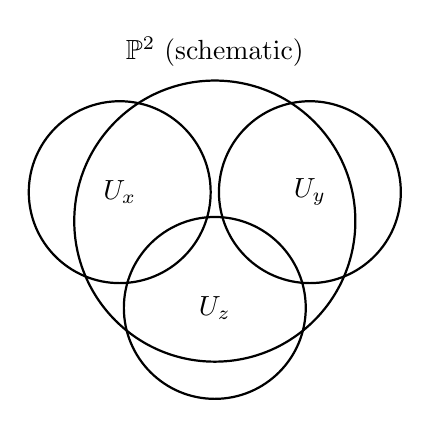
\begin{tikzpicture}[scale=1.05, line cap=round, line join=round]
		\draw[thick] (0,0) circle (1.7);
		\node at (0,2.05) {\(\mathbb P^2\) (schematic)};
		\draw[thick] (-1.15,0.35) circle (1.1);
		\draw[thick] (1.15,0.35) circle (1.1);
		\draw[thick] (0,-1.05) circle (1.1);
		\node at (-1.15,0.35) {\(U_x\)};
		\node at (1.15,0.35) {\(U_y\)};
		\node at (0,-1.05) {\(U_z\)};
	\end{tikzpicture}
	\caption{The standard affine cover \(\mathbb P^2=U_x\cup U_y\cup U_z\) (schematic).}
\end{figure}

\begin{figure}[h]
	\centering
	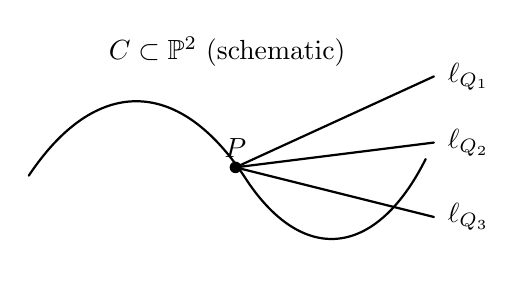
\begin{tikzpicture}[scale=1.05, line cap=round, line join=round]
		\draw[thick] (-2.4,0) .. controls (-1.6,1.2) and (-0.6,1.2) .. (0.2,0)
		.. controls (0.9,-1.1) and (1.8,-1.0) .. (2.4,0.2);
		\node at (0,1.5) {\(C\subset\mathbb P^2\) (schematic)};
		\fill (0.1,0.1) circle (2pt);
		\node[above] at (0.1,0.1) {\(P\)};
		\draw[thick] (0.1,0.1) -- (2.5,1.2);
		\draw[thick] (0.1,0.1) -- (2.5,0.4);
		\draw[thick] (0.1,0.1) -- (2.5,-0.5);
		\node[right] at (2.55,1.2) {\(\ell_{Q_1}\)};
		\node[right] at (2.55,0.4) {\(\ell_{Q_2}\)};
		\node[right] at (2.55,-0.5) {\(\ell_{Q_3}\)};
	\end{tikzpicture}
	\caption{Projection from \(P\): points of \(\mathbb P^1\) correspond to lines through \(P\).}
\end{figure}


\subsection*{Explicit local formulas for projection from \(P\) in Problem 9}

Let \(P\in \mathbb P^2\) and choose two independent linear forms
\[
\ell_0(x,y,z),
\qquad
\ell_1(x,y,z),
\]
such that
\[
\ell_0(P)=0,
\qquad
\ell_1(P)=0.
\]
Then the pencil of lines through \(P\) is precisely the family
\[
Z\bigl(\lambda \ell_0+\mu \ell_1\bigr),
\qquad
[\lambda:\mu]\in \mathbb P^1.
\]
The projection from \(P\) is the rational map
\[
\pi_P:\mathbb P^2\dashrightarrow \mathbb P^1,
\qquad
(x:y:z)\longmapsto \bigl(\ell_0(x,y,z):\ell_1(x,y,z)\bigr),
\]
which is undefined exactly at \(P\).
Restricting to the curve \(C\) gives a morphism
\[
\pi_P:C\to\mathbb P^1,
\]
because \(C\) is smooth and irreducible, so the indeterminacy point is removed by the restriction.

On an affine chart \(U_z=\{z\neq 0\}\) with coordinates
\[
x=\frac{x}{z},
\qquad
y=\frac{y}{z},
\]
and after a projective change of coordinates sending \(P\) to \((0:0:1)\), one can take
\[
\ell_0=x,
\qquad
\ell_1=y.
\]
Then the projection becomes
\[
\pi_P(x,y)=[x:y].
\]
On the chart \(\{x\neq 0\}\subset \mathbb P^1\) with affine coordinate \(m=y/x\), this is the slope map
\[
m=\frac{y}{x},
\]
and the fiber over \(m\in k\) is cut out by the line
\[
y=mx.
\]
The point \([1:0]\in\mathbb P^1\) corresponds to the vertical direction, whose fiber is cut out by
\[
x=0.
\]

\section*{Affine and projective spaces over a field \(k\)}

This chapter compares the basic ambient spaces used in algebraic geometry:
affine space
\(\mathbb A^n_k\)
and projective space
\(\mathbb P^n_k\).
We explain what their points are, how coordinates work, what the standard charts are, and what changes when
\[
k=\mathbb R
\quad\text{or}\quad
k=\mathbb C.
\]

\subsection*{Affine space \(\mathbb A^n_k\)}

\subsubsection*{Definition as a set and as a scheme}

As a set,
\[
\mathbb A^n_k = k^n.
\]
A point is an \(n\)-tuple
\[
(a_1,\dots,a_n).
\]

Algebraically,
\[
\mathbb A^n_k \simeq \operatorname{Spec} k[x_1,\dots,x_n].
\]
The polynomial ring
\[
k[x_1,\dots,x_n]
\]
is the coordinate ring of \(\mathbb A^n_k\).

\subsubsection*{Functions and morphisms}

Regular functions on \(\mathbb A^n_k\) are exactly polynomials:
\[
\Gamma(\mathbb A^n_k,\mathcal O)=k[x_1,\dots,x_n].
\]
A morphism
\[
f:\mathbb A^n_k\to\mathbb A^m_k
\]
is given by \(m\) polynomials
\[
f=(f_1,\dots,f_m),
\qquad
f_i\in k[x_1,\dots,x_n],
\]
via
\[
(a_1,\dots,a_n)\mapsto \bigl(f_1(a),\dots,f_m(a)\bigr).
\]

\subsubsection*{Closed sets in the Zariski topology}

A subset \(Z\subset \mathbb A^n_k\) is Zariski closed if it is the common zero set of polynomials:
\[
Z = Z(I)
=
\{a\in k^n : f(a)=0 \text{ for all } f\in I\},
\]
where \(I\subset k[x_1,\dots,x_n]\) is an ideal.
When \(k\) is algebraically closed, irreducible closed sets correspond to prime ideals.

\subsubsection*{Key examples}

\textbf{The affine line.}
\[
\mathbb A^1_k = k.
\]
Closed sets are finite subsets and all of \(\mathbb A^1_k\) (over an algebraically closed field).

\textbf{The affine plane.}
\[
\mathbb A^2_k = k^2.
\]
Typical curves are of the form
\[
Z(f(x,y))\subset \mathbb A^2_k,
\]
with \(f\in k[x,y]\).

\textbf{Affine \(n\)-space.}
\[
\mathbb A^n_k = k^n.
\]
It is the natural setting for polynomial equations in \(n\) variables.



\subsection*{Projective space \(\mathbb P^n_k\)}

\subsubsection*{Geometric definition: lines through the origin}

Projective \(n\)-space over \(k\) is the set of \(1\)-dimensional linear subspaces of \(k^{n+1}\):
\[
\mathbb P^n_k
=
\bigl\{
\text{lines } \ell \subset k^{n+1} \text{ through } 0
\bigr\}.
\]
Equivalently,
\[
\mathbb P^n_k
=
\bigl(k^{n+1}\setminus\{0\}\bigr)\big/\sim,
\]
where
\[
(x_0,\dots,x_n)\sim(\lambda x_0,\dots,\lambda x_n)
\]
for
\[
\lambda\in k^\times.
\]
A point is written in homogeneous coordinates as
\[
[x_0:\cdots:x_n].
\]

\subsubsection*{Algebraic definition: Proj of a graded ring}

Let
\[
S=k[x_0,\dots,x_n]
\]
with its standard grading by total degree.
Then
\[
\mathbb P^n_k \simeq \operatorname{Proj}(S).
\]
Homogeneous ideals in \(S\) define projective algebraic sets in \(\mathbb P^n_k\).

\subsubsection*{Standard affine charts}

For each \(i\in\{0,\dots,n\}\), define the standard open subset
\[
U_i=\{x_i\neq 0\}\subset \mathbb P^n_k.
\]
On \(U_i\) we use affine coordinates
\[
u_j=\frac{x_j}{x_i}
\quad\text{for } j\neq i,
\]
giving an isomorphism
\[
U_i \simeq \mathbb A^n_k.
\]
On overlaps \(U_i\cap U_j\), the transition functions are rational:
\[
\frac{x_\ell}{x_i}
=
\frac{x_\ell/x_j}{x_i/x_j}.
\]

\subsubsection*{Hyperplanes and the line at infinity}

A hyperplane in \(\mathbb P^n_k\) is the zero set of a nonzero linear homogeneous form
\[
a_0x_0+\cdots+a_nx_n.
\]
In particular, in \(\mathbb P^n_k\) the subset
\[
H_\infty = Z(x_0)
\]
is a hyperplane.
The complement is affine:
\[
\mathbb P^n_k\setminus Z(x_0)\simeq \mathbb A^n_k
\]
via
\[
[x_0:x_1:\cdots:x_n]\mapsto \left(\frac{x_1}{x_0},\dots,\frac{x_n}{x_0}\right).
\]
For \(n=2\), the hyperplane \(Z(x_0)\) is a \emph{projective line} and is often called the \emph{line at infinity}.

\subsubsection*{Why projective space is useful}

Projective space compactifies affine space by adding points at infinity.
Geometrically this eliminates many ``missing intersection'' phenomena.
For example, two distinct lines in \(\mathbb A^2_k\) can be parallel and disjoint, but their projective closures in \(\mathbb P^2_k\) always meet in exactly one point.

Projective space also treats homogeneous polynomials naturally.
If \(F\in k[x_0,\dots,x_n]\) is homogeneous, then the vanishing locus
\[
Z(F)\subset \mathbb P^n_k
\]
is well-defined, because scaling a point scales \(F\) by a power.



\section*{Comparing \(\mathbb A^n_k\) and \(\mathbb P^n_k\)}

\subsubsection*{Coordinates: affine vs homogeneous}

In \(\mathbb A^n_k\) a point has coordinates \((a_1,\dots,a_n)\) with no scaling.
In \(\mathbb P^n_k\) coordinates are only defined up to a common nonzero scalar:
\[
[x_0:\cdots:x_n] = [\lambda x_0:\cdots:\lambda x_n].
\]

\subsubsection*{Affine space inside projective space}

Affine space is an open subset of projective space:
\[
\mathbb A^n_k \simeq U_0 = \{x_0\neq 0\}\subset \mathbb P^n_k.
\]
The complement
\[
\mathbb P^n_k\setminus \mathbb A^n_k
\]
is the hyperplane at infinity \(Z(x_0)\), which is isomorphic to \(\mathbb P^{n-1}_k\).

\subsubsection*{Homogenization and projective closure}

Given a polynomial \(f(x_1,\dots,x_n)\) of total degree \(d\), define its homogenization
\[
F(x_0,x_1,\dots,x_n)=x_0^d\,f\!\left(\frac{x_1}{x_0},\dots,\frac{x_n}{x_0}\right).
\]
Then \(F\) is homogeneous of degree \(d\), and the projective closure of the affine hypersurface \(Z(f)\subset \mathbb A^n_k\) is
\[
\overline{Z(f)} = Z(F)\subset \mathbb P^n_k.
\]
The points of \(\overline{Z(f)}\cap Z(x_0)\) are the points at infinity.

\subsubsection*{Lines and curves}

\textbf{Affine lines.}
An affine line in \(\mathbb A^n_k\) is a translate of a 1-dimensional subspace:
\[
\{a+tv : t\in k\},
\]
with \(a,v\in k^n\) and \(v\neq 0\).

\textbf{Projective lines.}
A projective line in \(\mathbb P^n_k\) is a copy of \(\mathbb P^1_k\), equivalently the projectivization of a 2-dimensional subspace of \(k^{n+1}\).
In \(\mathbb P^2_k\), every line is cut out by one linear equation.

\textbf{Curves.}
In \(\mathbb A^2_k\), curves are typically defined by one polynomial equation \(f(x,y)=0\).
In \(\mathbb P^2_k\), plane curves are defined by one homogeneous equation \(F(x,y,z)=0\).



\subsection*{Special cases: \(k=\mathbb R\) and \(k=\mathbb C\)}

\subsubsection*{Real affine and projective spaces}

\textbf{Real affine space.}
\[
\mathbb A^n_{\mathbb R}=\mathbb R^n
\]
with its usual Euclidean topology and smooth manifold structure.

\textbf{Real projective space.}
\[
\mathbb P^n_{\mathbb R}
=
\bigl(\mathbb R^{n+1}\setminus\{0\}\bigr)/\sim,
\]
where \((v)\sim(\lambda v)\) for \(\lambda\in\mathbb R^\times\).
Equivalently,
\[
\mathbb P^n_{\mathbb R}\simeq S^n/\{v\sim -v\}.
\]
So \(\mathbb P^n_{\mathbb R}\) is a real \(n\)-dimensional manifold.

Important examples:
\[
\mathbb P^1_{\mathbb R}\simeq S^1,
\]
\[
\mathbb P^2_{\mathbb R}\ \text{is a non-orientable surface}.
\]
A key geometric fact is that \(\mathbb P^2_{\mathbb R}\) cannot be embedded in \(\mathbb R^3\) without self-intersection, though it can be embedded in \(\mathbb R^4\).

\subsubsection*{Complex affine and projective spaces}

\textbf{Complex affine space.}
\[
\mathbb A^n_{\mathbb C}=\mathbb C^n
\]
is a complex \(n\)-dimensional manifold, hence real \(2n\)-dimensional.

\textbf{Complex projective space.}
\[
\mathbb P^n_{\mathbb C}
=
\bigl(\mathbb C^{n+1}\setminus\{0\}\bigr)/\sim,
\]
where \((v)\sim(\lambda v)\) for \(\lambda\in\mathbb C^\times\).
Topologically,
\[
\mathbb P^n_{\mathbb C}\simeq S^{2n+1}/S^1.
\]
So \(\mathbb P^n_{\mathbb C}\) is a complex \(n\)-dimensional manifold, hence real \(2n\)-dimensional.

Important examples:
\[
\mathbb P^1_{\mathbb C}\ \text{is the Riemann sphere},
\qquad
\mathbb P^1_{\mathbb C}\simeq S^2.
\]
Also,
\[
\mathbb P^2_{\mathbb C}
\ \text{has real dimension } 4,
\]
so it is not a surface in \(\mathbb R^3\).

\subsubsection*{Zariski topology versus Euclidean topology}

When \(k=\mathbb R\) or \(k=\mathbb C\), affine and projective spaces carry both:
the Zariski topology (from polynomial equations) and the usual Euclidean topology.
The Zariski topology is much coarser.
For example, in \(\mathbb A^1_{\mathbb C}\) the Zariski closed sets are finite sets and the whole space, whereas in the Euclidean topology there are many more closed sets.

In algebraic geometry, morphisms and regular functions are defined using the Zariski topology and polynomial or rational expressions, not using analytic continuity.



\subsection*{Quick reference table}

\begin{itemize}
	\item \(\mathbb A^n_k\) is \(k^n\) and equals \(\operatorname{Spec}k[x_1,\dots,x_n]\).
	\item Regular functions on \(\mathbb A^n_k\) are polynomials.
	\item \(\mathbb P^n_k\) is the set of lines through \(0\) in \(k^{n+1}\) and equals \(\operatorname{Proj}k[x_0,\dots,x_n]\).
	\item \(\mathbb P^n_k\) is covered by \(n+1\) affine charts \(U_i=\{x_i\neq 0\}\), each isomorphic to \(\mathbb A^n_k\).
	\item \(\mathbb A^n_k\) sits inside \(\mathbb P^n_k\) as \(\mathbb P^n_k\setminus Z(x_0)\), and \(Z(x_0)\simeq\mathbb P^{n-1}_k\) is the hyperplane at infinity.
	\item Over \(\mathbb R\), \(\mathbb P^n_{\mathbb R}\simeq S^n/\{v\sim -v\}\).
	\item Over \(\mathbb C\), \(\mathbb P^n_{\mathbb C}\simeq S^{2n+1}/S^1\).
\end{itemize}

\subsection*{Affine varieties, projective varieties, and quasi-affine varieties}

\subsubsection*{Affine algebraic sets and affine varieties}

A subset \(X\subset \mathbb A^n_k\) is an \emph{affine algebraic set} if there exists an ideal
\[
I\subset k[x_1,\dots,x_n]
\]
such that
\[
X=Z(I).
\]
The \emph{coordinate ring} of \(X\) is
\[
k[X]=k[x_1,\dots,x_n]/I(X),
\]
where \(I(X)\) is the ideal of all polynomials vanishing on \(X\).

An \emph{affine variety} means an affine algebraic set that is irreducible.
Equivalently, \(X\) is an affine variety if \(I(X)\) is a prime ideal.

\subsubsection*{Projective algebraic sets and projective varieties}

A subset \(Y\subset \mathbb P^n_k\) is a \emph{projective algebraic set} if it is the common zero locus of homogeneous polynomials:
\[
Y=Z(J)
\]
for some homogeneous ideal \(J\subset k[x_0,\dots,x_n]\).
A \emph{projective variety} means a projective algebraic set that is irreducible.

\subsubsection*{Quasi-affine varieties}

A \emph{quasi-affine} variety is an open subvariety of an affine variety.
Equivalently, it is a variety that can be realized as
\[
U = X\setminus Z
\]
where \(X\) is affine and \(Z\subset X\) is a closed subvariety.

Typical examples:
\[
\mathbb A^n_k\setminus Z(f)
\]
is quasi-affine for any polynomial \(f\), and in fact it is affine because it is the principal open set
\[
D(f)=\operatorname{Spec}k[x_1,\dots,x_n]_f.
\]

\subsubsection*{Example: \(\mathbb A^2_k\setminus\{0\}\) is quasi-affine but not affine}

Let
\[
U=\mathbb A^2_k\setminus\{(0,0)\}.
\]
Then \(U\) is quasi-affine because it is an open subset of \(\mathbb A^2_k\).

However, \(U\) is not affine.
Indeed, one has a cover
\[
U=D(x)\cup D(y),
\]
and a standard computation shows
\[
\Gamma(U,\mathcal O_U)=k[x,y].
\]
If \(U\) were affine, then
\[
U\simeq \operatorname{Spec}\Gamma(U,\mathcal O_U)=\operatorname{Spec}k[x,y]=\mathbb A^2_k,
\]
which is impossible because \(U\neq \mathbb A^2_k\).
So \(U\) is quasi-affine but not affine.

\subsubsection*{Projective space is not affine}

Projective space \(\mathbb P^n_k\) is not affine for \(n\ge 1\).
One reason is that every regular function on \(\mathbb P^n_k\) is constant:
\[
\Gamma(\mathbb P^n_k,\mathcal O)=k.
\]
In particular, \(\mathbb P^n_k\) cannot be isomorphic to \(\mathbb A^m_k\) for any \(m\).

\subsubsection*{Affine pieces inside projective varieties}

Every projective variety \(Y\subset \mathbb P^n_k\) is covered by affine charts.
For example,
\[
Y=\bigl(Y\cap U_0\bigr)\cup\cdots\cup\bigl(Y\cap U_n\bigr),
\]
and each \(Y\cap U_i\) is an affine variety defined by dehomogenizing the defining homogeneous equations on the chart \(U_i\).

%This is why one often studies projective varieties locally using affine coordinates, while keeping global projective geometry available for intersection arguments.

%\subsubsection*{Concrete examples: polynomials, ideals, coordinate rings, and quotients}

Throughout, let \(k\) be a field (often \(k=\mathbb R\) or \(k=\mathbb C\)).

\paragraph{Example A1: a point in \(\mathbb A^2\).}
Let
\[
X=\{(1,2)\}\subset \mathbb A^2_k.
\]
Then
\[
I(X)=(x-1,\;y-2)\subset k[x,y],
\]
and
\[
k[X]=k[x,y]/(x-1,\;y-2)\simeq k.
\]
This reflects that regular functions on a point are just constants.

\paragraph{Example A2: a line in \(\mathbb A^2\).}
Let
\[
X=Z(y-x)\subset \mathbb A^2_k.
\]
Then
\[
I(X)=(y-x),
\]
and
\[
k[X]=k[x,y]/(y-x)\simeq k[x]
\]
via the substitution \(y=x\).
So \(X\simeq \mathbb A^1_k\).

\paragraph{Example A3: a parabola in \(\mathbb A^2\).}
Let
\[
X=Z(y-x^2)\subset \mathbb A^2_k.
\]
Then
\[
I(X)=(y-x^2),
\]
and
\[
k[X]=k[x,y]/(y-x^2)\simeq k[x].
\]
Geometrically, \(X\) is isomorphic to \(\mathbb A^1_k\) via \(x\mapsto (x,x^2)\).

\paragraph{Example A4: a reducible affine curve.}
Let
\[
X=Z(xy)\subset \mathbb A^2_k.
\]
Then
\[
I(X)=(xy),
\]
and
\[
k[X]=k[x,y]/(xy).
\]
The curve \(X\) is the union of the coordinate axes
\[
Z(x)\cup Z(y),
\]
and the coordinate ring has zero divisors because
\[
\overline{x}\cdot \overline{y}=0
\]
in \(k[X]\).
Thus \(X\) is not an affine variety (it is not irreducible).

\paragraph{Example A5: an irreducible affine curve with a singularity.}
Let
\[
X=Z(y^2-x^3)\subset \mathbb A^2_k.
\]
Then
\[
I(X)=(y^2-x^3),
\]
and
\[
k[X]=k[x,y]/(y^2-x^3).
\]
Over \(\operatorname{char}(k)\neq 2,3\), this is irreducible (a cusp).
It is a variety but not smooth at the origin.

\paragraph{Example A6: a hypersurface in \(\mathbb A^3\).}
Let
\[
X=Z(x^2+y^2+z^2-1)\subset \mathbb A^3_k.
\]
Then
\[
I(X)=(x^2+y^2+z^2-1),
\]
and
\[
k[X]=k[x,y,z]/(x^2+y^2+z^2-1).
\]
For \(k=\mathbb R\) the real points form the usual sphere \(S^2\) as a subset of \(\mathbb R^3\),
while for \(k=\mathbb C\) the complex points form a complex surface in \(\mathbb C^3\).

\paragraph{Example P1: a projective point in \(\mathbb P^1\).}
Let
\[
p=[1:0]\in \mathbb P^1_k.
\]
Then
\[
p=Z(x_1)\subset \mathbb P^1_k,
\]
since \(x_1=0\) forces \([x_0:x_1]=[1:0]\).
Thus in \(\mathbb P^1\), a single linear equation cuts out a point.

\paragraph{Example P2: a projective line in \(\mathbb P^2\).}
Let
\[
L=Z(z)\subset \mathbb P^2_k.
\]
This is a projective line.
Its affine chart \(U_x=\{x\neq 0\}\) has coordinates \(Y=y/x\), \(Z=z/x\), and on this chart
\[
L\cap U_x=Z(Z)\subset \mathbb A^2_k,
\]
so \(L\cap U_x\simeq \mathbb A^1_k\).
Similarly on \(U_y\).
Globally,
\[
L\simeq \mathbb P^1_k.
\]

\paragraph{Example P3: a projective conic.}
Let
\[
C=Z(xz-y^2)\subset \mathbb P^2_k.
\]
On the chart \(U_z\) with \(X=x/z\), \(Y=y/z\), the equation becomes
\[
X-Y^2=0,
\]
so
\[
C\cap U_z\simeq Z(X-Y^2)\subset \mathbb A^2_k.
\]
The conic \(C\) is smooth, hence \(C\simeq \mathbb P^1_k\).

\paragraph{Example P4: projective closure of an affine curve.}
Consider the affine curve
\[
X=Z(y-x^2)\subset \mathbb A^2_k.
\]
Its projective closure in \(\mathbb P^2_k\) is obtained by homogenizing \(y-x^2\) to degree \(2\):
\[
F(x,y,z)=yz-x^2.
\]
Thus
\[
\overline{X}=Z(yz-x^2)\subset \mathbb P^2_k.
\]
The points at infinity are
\[
\overline{X}\cap Z(z)=Z(-x^2)\cap Z(z),
\]
so
\[
\overline{X}\cap Z(z)=\{[0:1:0]\}.
\]

\paragraph{Example Q1: a principal open subset is affine.}
Let
\[
U=\mathbb A^2_k\setminus Z(x)=D(x).
\]
Then \(U\) is affine and
\[
U\simeq \operatorname{Spec}k[x,y]_x,
\]
where
\[
k[x,y]_x
=
k[x,y]\left[\frac{1}{x}\right].
\]
So regular functions on \(U\) are polynomials in \(x,y\) allowing \(x^{-1}\).

\paragraph{Example Q2: removing a point from \(\mathbb A^2\).}
Let
\[
U=\mathbb A^2_k\setminus\{(0,0)\}.
\]
Then \(U\) is quasi-affine because it is open in \(\mathbb A^2_k\).
It is covered by two principal affines:
\[
U=D(x)\cup D(y).
\]
On this open set one has
\[
\Gamma(U,\mathcal O_U)=k[x,y].
\]
If \(U\) were affine, then \(U\simeq \operatorname{Spec}k[x,y]=\mathbb A^2_k\), which is false.
So \(U\) is quasi-affine but not affine.

\paragraph{Example Q3: affine pieces of projective space.}
Let
\[
U_z=\mathbb P^2_k\setminus Z(z).
\]
Then \(U_z\) is affine and
\[
U_z\simeq \mathbb A^2_k
\]
via
\[
[x:y:z]\mapsto \left(\frac{x}{z},\frac{y}{z}\right).
\]
The complement
\[
Z(z)\simeq \mathbb P^1_k
\]
is the line at infinity for this chart.

\paragraph{Example Q4: complement of a projective curve is quasi-affine.}
If \(C\subset \mathbb P^2_k\) is a projective plane curve, then
\[
\mathbb P^2_k\setminus C
\]
is quasi-affine, because it is an open subset of the projective variety \(\mathbb P^2_k\).
On standard charts \(U_x,U_y,U_z\), the intersections \((\mathbb P^2_k\setminus C)\cap U_i\) are affine opens of \(\mathbb A^2_k\).

\subsubsection*{Quick guide: reading quotients \(k[x_1,\dots,x_n]/I\)}

If \(I=(f_1,\dots,f_r)\), then in the quotient ring
\[
k[x_1,\dots,x_n]/I
\]
the relations
\[
f_1=\cdots=f_r=0
\]
hold identically.
For example, in
\[
k[x,y]/(y-x^2),
\]
one may replace every occurrence of \(y\) by \(x^2\), which explains the isomorphism with \(k[x]\).
In
\[
k[x,y]/(xy),
\]
the classes \(\overline{x}\) and \(\overline{y}\) are nonzero but satisfy \(\overline{x}\,\overline{y}=0\), so the ring has zero divisors and the variety is reducible.

\subsubsection*{Understanding \(I(X)=(x-1,y-2)\) and \(k[X]\simeq k\), plus the line example}

\textbf{A point in \(\mathbb A^2_k\).}
Let
\[
X=\{(1,2)\}\subset \mathbb A^2_k.
\]
The ideal \(I(X)\subset k[x,y]\) is defined by
\[
I(X)=\{f\in k[x,y] : f(1,2)=0\}.
\]

\textbf{Claim.}
\[
I(X)=(x-1,\;y-2).
\]

\textbf{Proof.}
First, \(x-1\) and \(y-2\) vanish at \((1,2)\), hence
\[
(x-1,\;y-2)\subset I(X).
\]
Conversely, let \(f\in k[x,y]\). Write
\[
f(x,y)-f(1,2)
=
\bigl(f(x,y)-f(1,y)\bigr)
+
\bigl(f(1,y)-f(1,2)\bigr).
\]
For the first difference, treat \(y\) as a parameter and factor \(x-1\):
\[
f(x,y)-f(1,y)=(x-1)\,A(x,y)
\]
for some \(A\in k[x,y]\).
For the second difference, treat \(x=1\) as fixed and factor \(y-2\):
\[
f(1,y)-f(1,2)=(y-2)\,B(y)
\]
for some \(B\in k[y]\subset k[x,y]\).
Therefore
\[
f(x,y)-f(1,2)=(x-1)A(x,y)+(y-2)B(y).
\]
If \(f(1,2)=0\), then
\[
f(x,y)=(x-1)A(x,y)+(y-2)B(y),
\]
so \(f\in (x-1,y-2)\). Hence
\[
I(X)\subset (x-1,y-2),
\]
and the claim follows.

\textbf{Coordinate ring and why it is \(k\).}
The coordinate ring of \(X\) is
\[
k[X]=k[x,y]/I(X)=k[x,y]/(x-1,y-2).
\]
In the quotient ring the relations
\[
x-1=0,
\qquad
y-2=0
\]
hold, so one can replace \(x\) by \(1\) and \(y\) by \(2\).
Thus every polynomial class is determined by its value at \((1,2)\).

Formally, consider the evaluation homomorphism
\[
\operatorname{ev}_{(1,2)}:k[x,y]\to k,
\qquad
f\mapsto f(1,2).
\]
Its kernel is
\[
\ker(\operatorname{ev}_{(1,2)})=(x-1,y-2)=I(X),
\]
and its image is all of \(k\) because constants occur as values.
By the first isomorphism theorem,
\[
k[x,y]/(x-1,y-2)\simeq k.
\]

\bigskip

\textbf{The same idea on a line.}
Let
\[
L=Z(y-x)\subset \mathbb A^2_k.
\]
Then
\[
I(L)=(y-x),
\]
and the coordinate ring is
\[
k[L]=k[x,y]/(y-x).
\]
Inside this quotient we have the relation
\[
y=x,
\]
so every polynomial class can be rewritten using only \(x\).
Define a homomorphism
\[
\Phi:k[x,y]\to k[x],
\qquad
\Phi\bigl(f(x,y)\bigr)=f(x,x).
\]
Then
\[
\ker(\Phi)=(y-x),
\]
and \(\Phi\) is surjective.
Therefore, again by the first isomorphism theorem,
\[
k[x,y]/(y-x)\simeq k[x].
\]
Geometrically this says the line \(L\) is isomorphic to \(\mathbb A^1_k\), with coordinate \(x\).

\subsubsection*{Quotients by \((x-1)\) and evaluation at \(x=1\)}

\textbf{One variable.}
Consider the ideal
\[
(x-1)\subset k[x].
\]
Two polynomials \(f,g\in k[x]\) define the same class in the quotient ring
\[
k[x]/(x-1)
\]
if and only if their difference lies in \((x-1)\):
\[
f\equiv g \pmod{(x-1)}
\quad\Longleftrightarrow\quad
f-g\in (x-1).
\]
This is equivalent to saying that \(f\) and \(g\) have the same value at \(x=1\).
Indeed, if \(f-g\in(x-1)\), then
\[
f-g=(x-1)h
\]
for some \(h\in k[x]\), hence
\[
(f-g)(1)=0,
\]
so
\[
f(1)=g(1).
\]
Conversely, if \(f(1)=g(1)\), then \((f-g)(1)=0\), so \(x-1\) divides \(f-g\), which means
\[
f-g\in(x-1).
\]
Therefore,
\[
f\equiv g \pmod{(x-1)}
\quad\Longleftrightarrow\quad
f(1)=g(1).
\]

Equivalently, the evaluation homomorphism
\[
\operatorname{ev}_1:k[x]\to k,
\qquad
f\mapsto f(1),
\]
has kernel
\[
\ker(\operatorname{ev}_1)=(x-1),
\]
so by the first isomorphism theorem
\[
k[x]/(x-1)\simeq k.
\]

\textbf{Two variables.}
Similarly, for
\[
(x-1,\;y-2)\subset k[x,y],
\]
one has
\[
f\equiv g \pmod{(x-1,y-2)}
\quad\Longleftrightarrow\quad
f(1,2)=g(1,2).
\]

\subsubsection*{Projective zero loci: what are they subsets of?}

Let
\[
S=k[x_0,\dots,x_n]
\]
be the graded polynomial ring, graded by total degree.

\textbf{Homogeneous points.}
A point of projective space is an equivalence class
\[
[x_0:\cdots:x_n]\in \mathbb P^n_k
\]
of a nonzero vector \((x_0,\dots,x_n)\in k^{n+1}\setminus\{0\}\), where
\[
(x_0,\dots,x_n)\sim (\lambda x_0,\dots,\lambda x_n)
\]
for \(\lambda\in k^\times\).

\textbf{Why homogeneous polynomials.}
If \(F\in S\) is homogeneous of degree \(d\), then
\[
F(\lambda x_0,\dots,\lambda x_n)=\lambda^d\,F(x_0,\dots,x_n).
\]
Hence the condition
\[
F(x_0,\dots,x_n)=0
\]
is invariant under scaling, so it defines a well-defined condition on the projective point \([x_0:\cdots:x_n]\).

\textbf{Projective algebraic set.}
Given a homogeneous ideal
\[
J\subset S,
\]
its projective zero locus is the subset
\[
Z_{\mathbb P}(J)
=
\bigl\{
[x_0:\cdots:x_n]\in \mathbb P^n_k
:
F(x_0,\dots,x_n)=0 \text{ for all } F\in J
\bigr\}.
\]
So a homogeneous ideal defines a Zariski closed subset
\[
Z_{\mathbb P}(J)\subset \mathbb P^n_k.
\]

\textbf{Examples in \(\mathbb P^2\).}
A line is
\[
Z_{\mathbb P}(z)=\{[x:y:z]\in\mathbb P^2 : z=0\}.
\]
A point, for example \([1:0:0]\), is
\[
Z_{\mathbb P}(y,z)=\{[x:y:z]\in\mathbb P^2 : y=0,\ z=0\}.
\]

\textbf{Homogeneous coordinate ring.}
If
\[
Y=Z_{\mathbb P}(J)\subset \mathbb P^n_k,
\]
the associated graded ring
\[
S_Y=S/J
\]
is called the \emph{homogeneous coordinate ring} of \(Y\).
It is not the same thing as the ring of global regular functions on \(Y\).
For instance, on projective space one has
\[
\Gamma(\mathbb P^n_k,\mathcal O)=k,
\]
so global regular functions are constant.

\textbf{Relation to affine charts (dehomogenization).}
Let
\[
U_i=\{x_i\neq 0\}\subset \mathbb P^n_k,
\qquad
U_i\simeq \mathbb A^n_k.
\]
On \(U_i\) set
\[
u_j=\frac{x_j}{x_i}
\quad\text{for } j\neq i.
\]
If \(F\) is homogeneous of degree \(d\), define its dehomogenization on \(U_i\) by
\[
F_i(u)=F(u_0,\dots,1,\dots,u_n),
\]
meaning we divide by \(x_i^d\) and set \(x_i=1\).
Then
\[
Y\cap U_i
\]
is the affine algebraic set in \(\mathbb A^n_k\) cut out by the dehomogenized equations \(F_i\).

\textbf{Warning about ideals: saturation.}
Different homogeneous ideals can define the same projective subset.
The projectively relevant ideal is the saturation with respect to the irrelevant ideal
\[
\mathfrak m=(x_0,\dots,x_n).
\]
One has
\[
Z_{\mathbb P}(J)=Z_{\mathbb P}(J^{\mathrm{sat}}),
\]
where \(J^{\mathrm{sat}}\) removes components supported at the origin of \(k^{n+1}\).


	\end{document}
